\documentclass[10pt, a4paper]{report}
%%%%%%%%%%%%%%%%%%%%%%%% INPUT %%%%%%%%%%%%%%%%%%%%%%%%
\usepackage[utf8]{inputenc}
\usepackage[german]{babel}

%MATHEMATIK
\usepackage{amssymb}
\usepackage{amsmath}
\usepackage{cancel}
\usepackage{enumerate}
\usepackage{esint}
\DeclareMathOperator{\arsinh}{arsinh}
\DeclareMathOperator{\arccot}{arccot}

%LAYOUT
\usepackage[T1]{fontenc}
\usepackage{charter}
\usepackage{float}
\usepackage[margin=1cm, justification=centering, singlelinecheck=no,tablename=Tab., figurename=Abb.]{caption}
\usepackage{comment}
\usepackage{graphicx}
%\usepackage{hyperref}
\usepackage{xcolor}
\usepackage{wrapfig}

% BOLD
\let\oldtextbf\textbf
\renewcommand{\textbf}[1]{\textcolor{cyan}{\oldtextbf{#1}}}

% COLORS
\usepackage{sectsty}
\chapterfont{\color{cyan}}
\sectionfont{\color{orange}}
\subsectionfont{\color{blue}}
\subsubsectionfont{\color{violet}}

% BOXED
\newcommand*{\boxedcolor}{orange}
\makeatletter
\renewcommand{\boxed}[1]{\textcolor{\boxedcolor}{%
  \fbox{\normalcolor\m@th$\displaystyle#1$}}}

%%%%%%%%%%%%%%%%%%%%%%%% LSTLISTINGS %%%%%%%%%%%%%%%%%%%%%%%%
\usepackage{listings}
\lstset{numbers=left, numberstyle=\tiny, numbersep=10pt} \lstset{language=Java} % Code einbinden

\lstdefinestyle{customc}{
  belowcaptionskip=1\baselineskip,
  breaklines=true,
  frame=L,
  xleftmargin=\parindent,
  language=C,
  showstringspaces=false,
  basicstyle=\footnotesize\ttfamily,
  keywordstyle=\bfseries\color{green!40!black},
  commentstyle=\itshape\color{purple!40!black},
  identifierstyle=\color{blue},
  stringstyle=\color{orange},
}

\lstdefinestyle{customasm}{
  belowcaptionskip=1\baselineskip,
  frame=L,
  xleftmargin=\parindent,
  language=[x86masm]Assembler,
  basicstyle=\footnotesize\ttfamily,
  commentstyle=\itshape\color{purple!40!black},
}

\lstset{escapechar=@,style=customc}

% DOCUMENT
\begin{document}
\chapter{MATLAB Einstieg}
\section{Darstellungsformen einer komplexe Zahlen}
\subsection{Die Kartesische Form}
Eine komplexe Zahl $z$ lässt sich in der Gaussschen Zahlenebene durch einen Bildpunkt $P\left(z\right)$ oder durch einen vom Koordinatenursprung $O$ zum Bildpunkt $P\left(z\right)$ gerichteten Zeiger bildlich darstellen. Die komplexe Zahl besteht aus einem reellen $\text{Re}\left(z\right)=a$, einem imaginären Anteil $\text{Im}\left(z\right)=b$ und eine imaginäre Einheit $\text{j}^2=-1$. Die Menge ist $\mathbb{C}=\left\{z\,\vert\, z=a+\text{j}b\quad\,\text{ mit }a,b\in \mathbb{R}\right\}$
\begin{equation}
\boxed{z=a+\text{j}\,b}
\end{equation}
Die Länge des Zeigers heisst Betrag $\Big\vert z\Big\vert$ der komplexen Zahl $z$. 
\begin{equation}
\boxed{\Big\vert z\Big\vert=\sqrt{a^2+b^2}}
\end{equation}
Zwei komplexe Zahlen $z_1$ und $z_2$ sind genau gleich, $z_1=z_2$, wenn ihre Bildpunkte zusammenfallen, d.h. $a_1=a_2$ und $b_1=b_2$ ist.
\newline\newline
Die zu $z$ konjugiert komplexe Zahl $\overline{z}$ liegt spiegelsymmetrisch zur rellen Achse. Die komplexe Zahl $z$ und ihre konjugiert $\overline{z}$ unterscheiden sich in ihrem Imaginärteil durch das Vorzeichen.
\begin{equation}
\boxed{\overline{z}=\overline{a+\text{j}b}=a-\text{j}b}
\end{equation}
Somit gelten folgende Ausdrücke
\begin{enumerate}[$(i)$]
\item $\text{Re}\left(\overline{z}\right)=\text{Re}\left(z\right)=a$
\item $\Big\vert \overline{z}\Big\vert=\Big\vert z\Big\vert$
\item $\overline{\left(\overline{z}\right)}=z$
\item Gilt $\overline{z}=z$, so ist $z$ reell
\end{enumerate}
%%%%%%%%%%%%%%%%%%%%%%%%%%%%%%%%%%%%%%%%%%%%%%%%%%%%%%%%%%%%%%%%%%%%%%%%%%%%%%%%%
\subsection{Die Polarform}
In der Polarform erfolgt die Darstellung einer komplexen Zahl durch die Polarkoordinaten $r$ und $\varphi$. Man beschränkt sich auf $\left[0,2\pi\right)$.
\begin{equation}
\boxed{r=\sqrt{a^2+b^2}}\quad \boxed{\varphi=\arctan\left(\dfrac{b}{a}\right)+\left\{\begin{array}{l}+0,\quad \text{(I)}\\+\pi,\quad \text{(II, III)}\\+2\pi,\quad \text{(IV)}\end{array}\right\}}
\end{equation}
Die \textbf{goniometrische Form} besteht aus dem Betrag und dem Argument von $z$. Die entsprechende konjugiert komplexe Zahl ist
\begin{equation}
\boxed{z=r\cdot \Big(\cos\left(\varphi\right)+\text{j}\sin\left(\varphi\right)\Big)}\quad 
\boxed{\overline{z}=r\cdot \Big(\cos\left(\varphi\right)-\text{j}\sin\left(\varphi\right)\Big)}
\end{equation}
Die \textbf{Exponentialform} besteht aus dem Betrag und dem Argument von $z$. Die entsprechende konjugierte komplexe Zahl ist
\begin{equation}
\boxed{z=r\cdot e^{\text{j}\varphi}}\quad
\boxed{\overline{z}=r\cdot e^{-\text{j}\varphi}}
\end{equation}
Somit ergeben sich folgende Beziehungen
\begin{equation}
\boxed{e^{\text{j}\varphi}=\cos\left(\varphi\right)+\text{j}\sin\left(\varphi\right)}\quad \boxed{e^{-\text{j}\varphi}=\cos\left(\varphi\right)-\text{j}\sin\left(\varphi\right)}
\end{equation}
\section{Grundrechenarten für komplexe Zahlen}
\subsection{Addition und Subtraktion komplexer Zahlen}
Zwei komplexe Zahlen werden addiert bzw. subtrahiert, indem man ihre Real- und Imaginärteil (jeweils für sich getrennt) addiert bzw. subtrahiert. Addition und Subtraktion sind nur in der karteischen Form durchführbar. Geometrisch entspricht dem Parallelogramregel der Vektorrechnung.  
\begin{equation}
\boxed{\begin{array}{lll}
z_1\pm z_2&=&\left(a_1+ \text{j}b_1\right)\pm \left(a_2+ \text{j}b_2\right)\\
&=&\left(a_1\pm a_2\right)+\text{j}\left(b_1\pm b_2\right)
\end{array}}
\end{equation}
\begin{enumerate}[$(i)$]
\item $z_1+z_2=z_2+z_1$
\item $z_1+\left(z_2+z_3\right)=\left(z_1+z_2\right)+z_3$
\end{enumerate}
\subsection{Multiplikation komplexer Zahlen}
Die Multiplikation in \textbf{kartesische Form} erfolgt, indem jeder Summand der ersten Klammer mit jedem Summand der zweiter Klammer unter Beachtung von $\text{j}^2=-1$ multipliziert. Geometrisch erfolgt eine Drehung im Gegenuhrzeigersinn falls $\varphi_2>0$ und im Uhrzeigersinn falls $\varphi_2<0$ und eine Streckung um den Faktor $r_2$. 
\begin{equation}
\boxed{\begin{array}{lll}
z_1\cdot z_2&=&\left(a_1+\text{j}b_1\right)\cdot \left(a_2+\text{j}b_2\right)\\
&=&\left(a_1a_2-b_1b_2\right)+\text{j}\left(a_1b_2+a_2b_1\right)
\end{array}}
\end{equation}
Die Multiplikation in \textbf{Polarform} erfolgt, indem man ihre Beträge multipliziert und die Argumente addiert.
\begin{equation}
\boxed{\begin{array}{lll}
z_1\cdot z_2&=&\Big[r_1\Big(\cos\left(\varphi_1\right)+\text{j}\sin\left(\varphi_1\right)\Big)\Big]\cdot r_2\Big(\cos\left(\varphi_2\right)+\text{j}\sin\left(\varphi_2\right)\Big)\Big]\\
&=&\left(r_1r_2\right)\cdot \Big[\cos\left(\varphi_1+\varphi_2\right)+\text{j}\sin\left(\varphi_1+\varphi_2\right)\Big]
\end{array}}
\end{equation}
\begin{equation}
\boxed{\begin{array}{lll}
z_1\cdot z_2&=&\Big(r_1\cdot e^{\text{j}\varphi_1}\Big)\cdot \Big(r_2\cdot e^{\text{j}\varphi_2}\Big)\\
&=&\left(r_1r_2\right)\cdot e^{\text{j}\left(\varphi_1+\varphi_2\right)}
\end{array}}
\end{equation}
\begin{enumerate}[$(i)$]
\item $z_1z_2=z_2z_1$
\item $z_1\left(z_2z_3\right)=\left(z_1z_2\right)z_3$
\item $z_1\left(z_2+z_3\right)=z_1z_2+z_1z_3$
\item $z\cdot \overline{z}=a^2+b^2=\Big\vert z\Big\vert^2\Longrightarrow \Big\vert z\Big\vert=\sqrt{z\cdot \overline{z}}$
\item $\text{j}^{4n}=1,\quad \text{j}^{4n+1}=\text{j},\quad \text{j}^{4n+2}=-1,\quad \text{j}^{4n+3}=-\text{j}\quad \left(n\in \mathbb{Z}\right)$
\end{enumerate}
\subsection{Division komplexer Zahlen}
Zähler und Nenner des Quotienten  werden zunächst mit dem konjugiert komplexen Nenner, d.h. der Zahl $\overline{z}_2$ multipliziert, dadurch wird der Nenner reell. Geometrisch erfährt $z_1$ eine Zurückdrehung im Uhrzeigersinn falls $\varphi_2>0$ und im Gegenuhrzeigersinn falls $\varphi_2<0$ und eine Streckung um den Faktor $1/r_2$.
\begin{equation}
\boxed{
\begin{array}{lll}
\dfrac{z_1}{z_2}&=&\dfrac{a_1+\text{j}b_1}{a_2+\text{j}b_2}=\dfrac{\left(a_1+\text{j}b_1\right)\cdot \left(a_2+\text{j}b_2\right)}{\left(a_2+\text{j}b_2\right)\cdot \left(a_2+\text{j}b_2\right)}\\\\
&=&\dfrac{a_1a_2+b_1b_2}{a_2^2+b_2^2}+\text{j}\dfrac{a_2b_1-a_1b_2}{a_2^2+b_2^2}
\end{array}
}
\end{equation}
\begin{equation}
\boxed{
\begin{array}{lll}
\dfrac{z_1}{z_2}&=&\dfrac{r_1\Big[\cos\left(\varphi_1\right)+\text{j}\sin\left(\varphi_1\right)\Big]}{r_2\Big[\cos\left(\varphi_2\right)+\text{j}\sin\left(\varphi_2\right)\Big]}\\
&=&\left(\dfrac{r_1}{r_2}\right)\cdot \Big[\cos\left(\varphi_1-\varphi_2\right)+\text{j}\sin\left(\varphi_1-\varphi_2\right)\Big]
\end{array}
}
\end{equation}
\begin{equation}
\boxed{\begin{array}{lll}
\dfrac{z_1}{z_2}&=&\dfrac{r_1\cdot e^{\text{j}\varphi_1}}{r_2\cdot e^{\text{j}\varphi_2}}=\left(\dfrac{r_1}{r_2}\right)\cdot e^{\text{j}\left(\varphi_1-\varphi_2\right)}\end{array}}
\end{equation}
\begin{enumerate}[$(i)$]
\item $\dfrac{1}{z}=\dfrac{1}{r\cdot e^{\text{j}\varphi}}=\left(\dfrac{1}{r}\right)\cdot e^{-\text{j}\varphi}$
\item $\dfrac{1}{z}=\dfrac{1}{a+\text{j}b}=\dfrac{a}{a^2+b^2}-\text{j}\dfrac{b}{a^2+b^2}$
\item $\dfrac{1}{\text{j}}=-\text{j}$
\end{enumerate}
\section{Potenzieren komplexer Zahlen}
\subsection{Die kartesische Form}
In \textbf{kartesischer Form} ist das Potenzieren komplexer Zahlen nach dem binomischen Lehrsatz  
\begin{equation}
\boxed{z^n=\left(a+\text{j}b\right)^n=a^n+\text{j}\displaystyle \binom{n}{1}a^{n-1}b+\text{j}^2\displaystyle\binom{n}{2}a^{n-2}b^2+\dotso+\text{j}^nb^n}
\end{equation}
\subsection{Die Polarform}
In \textbf{Polarform} wird der Betrag in die $n$-te Potenz erhebt und ihr Argument mit dem Exponenten $n$ multipliziert
\begin{equation} 
\boxed{
\begin{array}{lll}
z^n&=&\Big[r\cdot \Big(\cos\left(\varphi\right)+\text{j}\sin\left(\varphi\right)\Big)\Big]^n\\\\
&=&r^n\cdot \Big[\cos\left(n\varphi\right)+\text{j}\sin\left(n\varphi\right)\Big]
\end{array}
}
\end{equation} 
\begin{equation}
\boxed{
\begin{array}{lll}
z^n&=&\Big[r\cdot e^{\text{j}\varphi}\Big]^n=r^n\cdot e^{\text{j}n\varphi}
\end{array}
} 
\end{equation} 
\section{Radizieren komplexer Zahlen}
Eine komplexe Zahl $z$ heisst eine $n$-te Wurzel aus $a$, wenn sie der algebraischen Gleichung $z^n=a$ genügt $\left(a\in\mathbb{C};\quad n\in \mathbb{N}^*\right)$.
\newline\newline
Eine algebraische Gleichung $n$-ten Grades von folgendem Typ besitzt in der Menge $\mathbb{C}$ der komplexen Zahlen stets genau $n$ Lösungen. Bei ausschliesslich reellen koeffizienten $a_i$ treten komplexe Lösungen immer paarweise in Form konjugiert komplexer Zahlen auf.
\begin{equation}
\boxed{a_nz^n+a_{n-1}z^{n-1}+\dotso + a_1z+a_0=0,\quad \left(a_i:\,\text{reell oder komplex}\right)}
\end{equation}
Die $n$ Wurzeln der Gleichung $z^n=a=a_0\cdot e^{\text{j}\varphi}$ mit $a_0>0$ und $n\in \mathbb{N}^*$ lauten
\begin{equation}
\boxed{z_k=\sqrt[n]{a_0}\cdot \Big[\cos\left(\dfrac{\alpha+k\,2\pi}{n}\right)+\text{j}\sin\left(\dfrac{\alpha+k\,2\pi}{n}\right)\Big],\quad \left(k=0,\,1,\dotso, n-1\right)}
\end{equation}
Der Hauptwert ist bei $k=0$ und für $k=1, 2, \dotso, n-1$ erhält man Nebenwerte. Die Winkel können auch mîm Gradmass angegeben werden.
\newline\newline
geometrisch liegen die zugehörige Bildpunkte aufdem Mittelpunktskreis mit dem Radius $R=\sqrt[n]{a_0}$ und bilden die Ecken eines regelmässigen $n$-Ecks.
\newline\newline
Die $n$ Lösungen der Gleichung $z^n=1$ heissen $n$-te Einheitswurzeln und lauten
\begin{equation}
\boxed{z^n=1\Longrightarrow z_k=\cos\left(\dfrac{k\,2\pi}{n}\right)+\text{j}\sin\left(\dfrac{k\,2\pi}{n}\right)=e^{\text{j}\dfrac{k\,2\pi}{n}}}
\end{equation}
\section{Logarithmieren komplexer Zahlen}
Der natürliche Logarithmus einer komplexen Zahl 
\begin{equation}
\boxed{z=r\cdot e^{\text{j}\varphi}=r\cdot e^{\text{j}\left(\varphi+k\,2\pi\right)},\quad \left(0\leq \varphi< 2\pi;\,k\in \mathbb{Z}\right)}
\end{equation}
ist unendlich vieldeutig, denn der Hauptwert des Winkels wird häufig auch im Intervall $-\pi<\varphi < \pi$
\begin{equation}
\boxed{\ln\left(z\right)=\ln\left(r\right)+\text{j}\left(\varphi+k\,2\pi\right),\quad \left(k\in \mathbb{Z}\right)}
\end{equation}
\section{Ortskurven}
\subsection{Komplexwertige Funktion einer reellen Variablen}
Die von einem reellen Parameter $t$ abhängige komplexe Zahl heisst komplexwertige Funktion $z\left(t\right)$ der reellen Variablen $t$.
\begin{equation}
\boxed{z=z\left(t\right)=x\left(t\right)+\text{j}y\left(t\right),\quad \left(a\leq z\leq b\right)}
\end{equation}
\subsection{Ortskurve einer parameterabhängigen komplexen Zahl}
Die von einem parameterabhängigen komplexen Zeiger $\underline{z}=\underline{z}\left(t\right)$ in der Gaussschen Zahlenebene beschriebene Bahn heisst Ortskurve
\begin{equation}
\boxed{\underline{z}\left(t\right)=x\left(t\right)+\text{j}y\left(t\right)}
\end{equation}
\subsection{Inversion einer Ortskurve}
Der Übergang von einer komplexen Zahl $z\neq 0$ zu ihrem Kehrwert $w=1/z$ heisst Inversion. Vorzeichenwechsel im Argument, Kehrwertbildung des Betrages von $z$. Geometrisch wird der Zeiger an der reellen Achse gespiegelt und dann gestreckt mit Faktor $1/r^2$.
\begin{equation}
\boxed{z=r\cdot e^{\text{j}\varphi}\rightarrow w=\dfrac{1}{z}=\left(\dfrac{1}{r}\right)\cdot e^{-\text{j}\varphi}}
\end{equation}
\begin{enumerate}[$(i)$]
\item Der Punkt mit dem kleinsten Abstand vom Nullpunkt führt zu dem Bildpunkt mit dem grössten Abstand und umgekehrt.
\item Ein Punkt oberhalb der reellen Achse führt zu einem Bildpunkt unterhalb der reellen Achse und umgekehrt.
\item Eine Gerade durch den Nullpunkt auf der $z$-Ebene erzeugt eine Gerade durch den Nullpunkt auf der $w$-Ebene.
\item Eine Gerade, die nicht durch den Nullpunkt auf der $z$-Ebene geht, erzeugt einen Kreis durch den Nullpunkt auf der $w$-Ebene.
\item Ein Mittelpunktskreis auf der $z$-Ebene erzeugt einen Mittelpunktskreis auf der $w$-Ebene.
\item Ein Kreis durch den Nullpunkt auf der $z$-Ebene erzeugt eine Gerade, die nicht durch den Nullpunkt verläuft auf der $w$-Ebene.
\item Ein Kreis, der nicht durch den Nullpunkt auf der $z$-Ebene verläuft erzeugt einen Kreis, der nicht durch den Nullpunkt verläuft, auf der $w$-Ebene.
\end{enumerate}
\section{Komplexe Funktionen}
\subsection{Definition einer komplexen Funktion}
Unter der komplexen Funktion versteht man eine Vorschrift, de jeder komplexen Zahl $z\in D$ genau eine komplexe Zahl $w\in W$ zuordnet. Symbolische Schreibweise sind $w=f\left(z\right)$. $D$ und $W$ sind Teilmengen von $\mathbb{C}$.
\subsection{Definitionsgleichungen elementarer Funktionen}
\subsubsection{Trigonometrische Funktionen}
\begin{equation}
\boxed{\sin\left(z\right)=z-\dfrac{z^3}{3!}+\dfrac{z^5}{5!}-\dotso}
\quad
\boxed{\cos\left(z\right)=1-\dfrac{z^2}{4!}+\dfrac{z^4}{4!}-\dotso}
\end{equation}
\begin{equation}
\boxed{\tan\left(z\right)=\dfrac{\sin\left(z\right)}{\cos\left(z\right)}}
\quad
\boxed{\cot\left(z\right)=\dfrac{\cos\left(z\right)}{\sin\left(z\right)}=\dfrac{1}{\tan\left(z\right)}}
\end{equation}
\subsubsection{Hyperbelfunktionen}
\begin{equation}
\boxed{\sinh\left(z\right)=z+\dfrac{z^3}{3!}+\dfrac{z^5}{5!}-\dotso}
\quad
\boxed{\cosh\left(z\right)=1+\dfrac{z^2}{4!}+\dfrac{z^4}{4!}-\dotso}
\end{equation}
\begin{equation}
\boxed{\tanh\left(z\right)=\dfrac{\sinh\left(z\right)}{\cosh\left(z\right)}}
\quad
\boxed{\coth\left(z\right)=\dfrac{\cosh\left(z\right)}{\sinh\left(z\right)}=\dfrac{1}{\tanh\left(z\right)}}
\end{equation}
\subsubsection{Exponentialfunktion}
\begin{equation}
\boxed{e^z=1+\dfrac{z}{1!}+\dfrac{z^2}{2!}+\dfrac{z^3}{3!}+\dotso}
\end{equation}
\subsection{Beziehungen}
\subsubsection{Eulersche Formeln}
\begin{equation}
\boxed{e^{\text{j}x}=\cos\left(x\right)+\text{j}\sin\left(x\right)}
\quad
\boxed{e^{-\text{j}x}=\cos\left(x\right)-\text{j}\sin\left(x\right)}
\end{equation}
\subsubsection{Beziehungen trigonometrischen und komplexen $e$-Funktion}
\begin{equation}
\boxed{\sin\left(x\right)=\dfrac{1}{2\text{j}}\left(e^{\text{j}x}-e^{-\text{j}x}\right)}
\quad
\boxed{\cos\left(x\right)=\dfrac{1}{2}\left(e^{\text{j}x}+e^{-\text{j}x}\right)}
\end{equation}
\begin{equation}
\boxed{\tan\left(x\right)=-\text{j}\dfrac{\left(e^{\text{j}x}-e^{-\text{j}x}\right)}{\left(e^{\text{j}x}+e^{-\text{j}x}\right)}}
\quad
\boxed{\cot\left(x\right)=\text{j}\dfrac{\left(e^{\text{j}x}+e^{-\text{j}x}\right)}{\left(e^{\text{j}x}-e^{-\text{j}x}\right)}}
\end{equation}
\subsubsection{Beziehungen trigonometrischen und Hyperbelfunktionen}
\begin{equation}
\boxed{\sin\left(\text{j}x\right)=\text{j}\cdot \sinh\left(x\right)}\quad \boxed{\cos\left(\text{j}x\right)=\cosh\left(x\right)}\quad \boxed{\tan\left(\text{j}x\right)=\text{j}\cdot \tanh\left (x\right)}
\end{equation}
\begin{equation}
\boxed{\sinh\left(\text{j}x\right)=\text{j}\cdot \sin\left(x\right)}\quad \boxed{\cosh\left(\text{j}x\right)=\cos\left(x\right)}\quad \boxed{\tanh\left(\text{j}x\right)=\text{j}\cdot \tan\left (x\right)}
\end{equation}
\subsubsection{Additionstheoreme der trigonometrischen und Hyperbelfunktionen}
\begin{equation}
\boxed{\begin{array}{lll}
\sin\left(x\pm \text{j}y\right)&=&\sin\left(x\right)\cdot \cosh\left(y\right)\pm \text{j}\cdot \cos\left(x\right)\cdot \sinh\left(y\right)\\
\cos\left(x\pm \text{j}y\right)&=&\cos\left(x\right)\cdot \cosh\left(y\right)\mp \text{j}\cdot \sin\left(x\right)\cdot \sinh\left(y\right)\\
\tan\left(x\pm \text{j}y\right)&=&\dfrac{\sin\left(2x\right)\pm \text{j}\cdot \sinh\left(2x\right)}{\cos\left(2x\right)+\cosh\left(2x\right)}\\
\end{array}}
\end{equation}
\begin{equation}
\boxed{\begin{array}{lll}
\sinh\left(x\pm \text{j}y\right)&=&\sinh\left(x\right)\cdot \cos\left(y\right)\pm \text{j}\cdot \cosh\left(x\right)\cdot \sin\left(y\right)\\
\cosh\left(x\pm \text{j}y\right)&=&\cosh\left(x\right)\cdot \cos\left(y\right)\pm \text{j}\cdot \sinh\left(x\right)\cdot \sin\left(y\right)\\
\tanh\left(x\pm \text{j}y\right)&=&\dfrac{\sinh\left(2x\right)\pm \text{j}\cdot \sin\left(2x\right)}{\cosh\left(2x\right)+\cos\left(2x\right)}\\
\end{array}}
\end{equation}
\subsubsection{Arkus- und Areafunktionen}
\begin{equation}
\boxed{\arcsin\left(\text{j}x\right)=\text{j}\cdot \arsinh\left(x\right)}\quad \boxed{\arccos\left(\text{j}x\right)=\text{j}\cdot \text{Arcosh}\left(x\right)}
\end{equation}
\begin{equation}
\boxed{\arsinh\left(\text{j}x\right)=\text{j}\cdot \arcsin\left(x\right)}\quad \boxed{\text{Arcosh}\left(\text{j}x\right)=\text{j}\cdot \arccos\left(x\right)}
\end{equation}
\begin{equation}
\boxed{\arctan\left(\text{j}x\right)=\text{j}\cdot \text{Artanh}\left(x\right)}\quad \boxed{\text{Artanh}\left(\text{j}x\right)=\text{j}\cdot \arctan\left(x\right)}
\end{equation}
\section{Komplexe Zahlen in MATLAB}
\subsection{Definition der imaginäre Einheit}
Folgende Befehle sind Berechnungen der komplexen Zahlen
\begin{enumerate}[$\texttt{>}\texttt{>}$]
\item {\color{red}\texttt{sqrt(-1) => 0.0000 + 1.0000i}}
\item {\color{red}\texttt{i\^\,5 => 0.0000 + 1.0000i}}
\item {\color{red}\texttt{i\^\,10 => -1}}
\end{enumerate}
\subsection{Operationen mit komplexen Zahlen}
\begin{enumerate}[$\texttt{>}\texttt{>}$]
\item {\color{red}\texttt{double(solve('x\^\,2+x+1')) => -0.5000 + 0.8660i, -0.5000-0.8660i}}
\item {\color{red}\texttt{z1=3+4*i => 3.0000 + 4.0000i}}
\item {\color{red}\texttt{z2=complex(3,4) => 3.0000 + 4.0000i}} 
\item {\color{red}\texttt{real(z1) => 3}}
\item {\color{red}\texttt{imag(z1) => 4}}
\item {\color{red}\texttt{(3+4*i)+(1+2*i)/(-4+3*i) => 3.0800 + 3.5600i}}
\item {\color{red}\texttt{conj(1+2*i) => 1.0000 - 2.0000i}}
\item {\color{red}\texttt{(1+2*i)*conj(1+2*i) => 5}}
\end{enumerate}
\subsection{Gauss'sche Zahlenebene}
\begin{enumerate}[$\texttt{>}\texttt{>}$]
\item {\color{red}\texttt{plot([1+2*i,2-3*i,4-5*i,-3+i,i, -6, -3-2*i], 'r*')}}
\item {\color{red}\texttt{z=-2+i = -2.0000 + 1.0000i}}
\item {\color{red}\texttt{betrag=abs(z) => betrag =  2.2361}}
\item {\color{red}\texttt{sym=abs(z) => sym =  2.2361}}
\item {\color{red}\texttt{winkel=angle(z) => winkel =  2.6779}}
\item {\color{red}\texttt{winkel\_grad=winkel/pi*180 => winkel\_grad = 153.4349}}
\end{enumerate}
\subsection{Satz von Moivre}
\begin{enumerate}[$\texttt{>}\texttt{>}$]
\item {\color{red}\texttt{(-sqrt(3)-i)\^\,10 => 5.1200e+02 - 8.8681e+02i}}
\item {\color{red}\texttt{abs((-sqrt(3)-i)\^\,10) => 1.0240e+03}}
\item {\color{red}\texttt{angle((-sqrt(3)-i)\^\,10) => -1.0472}}
\item {\color{red}\texttt{(-sqrt(3)-i)\^\,(1/3) => 0.8099 - 0.9652i}}
\item {\color{red}\texttt{double(solve('z\^\,3-(-sqrt(3)-i)')) => 0.8099 - 0.9652i, -1.2408 - 0.2188i, 0.4309 + 1.1839i}}
\item {\color{red}\texttt{compass(double(solve('z\^\,3-(-sqrt(3)-i)')))}}
\end{enumerate}
\subsection{Eulersche Formel}
\begin{enumerate}[$\texttt{>}\texttt{>}$]
\item {\color{red}\texttt{log(-1) = 0.0000 + 3.1416i}}
\item {\color{red}\texttt{log(-10*i) = 2.3026 - 1.5708i}}
\item {\color{red}\texttt{log2(sqrt(2)-sqrt(2)*i) = 1.0000 - 1.1331i}}
\item {\color{red}\texttt{exp(1+i*pi) = -2.7183 + 0.0000i}}
\item {\color{red}\texttt{2\^i = 0.7692 + 0.6390i}}
\item {\color{red}\texttt{(-i)\^\,(-i) = 0.2079}}
\end{enumerate}
\chapter{Strahlung}
\section{Elemente der Programmiersprache Java}
\subsection{Bytecode}
Der Java-Compiler erzeugt aus den Quellcode-Dateien den so genannten \textbf{Bytecode}. Dieser Code ist binär und Ausgangspunkt für die virtuelle Machine zur Ausführung. Der Bytecode ist wie ein Prozessor, der Anweiungen wie arithmetische Operationen, Sprünge und Weiteres kennt.
\subsection{Java Virtual Machine}
Die Java Virtual Machine (JVM) kümmert sich um den Bytecode, den Quellcode auszuführen. Die Laufzeitumgebung lädt den Bytecode, prüft ihn und führt ihn in einer kontrollierten Umgebung aus. Java ist Plattform- und Betriebssystemunabhängig. Zu der JVM und der Programmiersprache kommen Standardbibliotheken für Datenstrukturen, Zeichenkettenverarbeitung, Datumverarbeitung, grafische Oberflächen, Ein- und Ausgabe, Netzwerkoperationen und mehr.
\subsection{Objektorientierung}
Eine Laufzeitumgebung eliminiert viele Fehler. Objektorientierte Programmierung versucht, die Komplexität des Softwareproblems besser zu modellieren. Menschen denken objektorientiert, darum Java bildet diese ab. Objekte bestehen aus \textbf{Eigenschaften}, also Dinge, die ein Objekt ``hat'' und ``kann''. Objekte entstehen aus \textbf{Klassen}, das sind Beschreibungen für den Aufbau von Objekten.
\\\\
Primitive Datentypen für numerische Zahlen oder Unicode-Zeichen werden nicht als Objekte betrachtet. Das \textbf{Java-Security-Modell} sicherstellt den Programmablauf. Der \textbf{Verifier} liest Code und überprüft die Korrektheit und Typsicherheit. Treten Sicherheitsprobleme auf, werden sie durch Exceptions zur Laufzeit gemeldet. Das Security-Manager überwächt Zugriffe auf das Dateisystem, die Netzwerk-Ports, externe Prozesse und weitere Systemressourcen.
\\\\
In Java gibt es keine Zeiger auf Speicherbereiche, dagegen führt Java \textbf{Referenzen} ein. Eine Referenz repräsentiert ein Objekt, und eine Variable speichert diese Referenz, sie wird Referenzvariable genannt. JVM verbindet die Referenz mit einem Speicherbereich und einem Referenztyp; der Zugriff, Dereferenzierung genannt, ist indirekt. Referenz und Speicherblock sind getrennt.
\\\\
In Java gibt es keine benutzerdefinierten überladenen Operatoren. Da das Operatorzeichen auf unterschiedlichen Datentypen gültig ist, nennt sich so ein Operator \textbf{Überladen}. Bei Zeichenketten werden Pluszeichen als \textbf{Konkatenation} angewendet. Java braucht keine \textbf{Präprozessoren}.
\subsection{Java Platform}
Mit dem Java Development Kit (JDK) lassen sich Java SE-Applikationen entwickeln. Dem JDK sind Hilfsprogramme beigelegt, die für die Java-Entwicklung nötig sind. Dazu zählen der essenzielle Compiler, aber auch andere Hilfsprogramme, etwa zur Signierung von Java-Archiven oder zum Start einer Management-Konsole.
\\\\
Das Java SE Runtime (JRE) enthält genau das, was zur Ausführung von Java-Programmen nötig ist. Die Distribution umfasst nur die JVM und Java-Bibliotheken, aber weder den Quellcode der Java-Bibliotheken noch Tools wie Management-Tools.
\subsection{Das erste Programm compilieren und testen}
\lstinputlisting[language=Java]{../../PROJEKTE/000001HelloWorld/src/Squares.java}
Ein Compiler übersetzt bzw. transformiert das geschriebene Programm in eine andere Repräsentation nämlich den Bytecode und erzeugt aus dem Program mit Endung \texttt{.java} die Datei \texttt{.class}, welche Bytecode enthält.
\\\\
Wenn der Compiler aufgrund eines syntaktischen Fehlers eine Übersetzung in Java-Bytecode nicht durchführen kann, spricht man von einem Compilerfehler.
\\\\
Eine Laufzeitumgebung liest die Bytecode-Datei Anweisung für Anweisung aus und führt sie auf den konkreten Mikroprozessor aus. Der Interpreter bringt das Programm zur Ausführung.
\\\\
Ein Java-Projekt braucht eine ordentliche Ordnerstruktur, und hier gibt es zur Organisation der Dateien unterschiedliche Ansätze. Die einfachste Form ist, Quellen, Klassendateien und Ressourcen in ein Verzeichnis zu setzen. Es gibt zwei Verzeichnisse \texttt{src} für die Quellen und \texttt{bin} für die erzeugten Klassendateien. Ein eigener Ordner \texttt{lib} ist sinnvoll für Java-Bibliotheken.
\\\\
Das Programm sitzt in einer Klasse, die drei Methoden enthält. Die Methode $\texttt{quadrat(int)}$, bekommt als Übergangsparameter eine ganze Zahl und berechnet daraus die Quadratzahl, die sie anschliessend zurückgibt. Eine weitere Methode übernimmt die Ausgabe der Quadratzahlen bis zu einer vorgegebenen Grenze. Die Methode \texttt{main()}, als Anfangspunkt, ruft die Methode \texttt{ausgabe(int)} auf.
\section{Imperative Sprachkonzepte}
\subsection{Elemente der Programmiersprache Java}
Unter dem Begriff \textbf{Semantik} versteht man die Lexikalik, Syntax und Semantik eines Programms. Der Compiler verläuft diese Schritte bevor er den Bytecode erzeugt.
\\\\
Ein \textbf{Token} ist eine lexikalische Einheit, die dem Compiler die Bausteine des Programms liefert. Der Compiler erkennt an der Grammatik einer Sprache, welche Folgen von Zeichen ein Token bilden.
\\\\
\textbf{Whitespaces} sind Leerzeichen, Tabulatoren, Zeilenvorschub und Seitenvorschubzeichen.
\\\\
Neben den Trennern gibt es noch zwölf ASCII-Zeichen geformte Tokens, die als \textbf{Separator} definiert werden: \texttt{( ) \{ \} [ ] ; , . ... @ ::}
\\\\
Für Variablen, Methoden, Klassen und Schnittstellen werden \textbf{Bezeichner}, auch \textbf{Identifizierer} genannt, vergeben. Unter \textbf{Variablen} sind dann Daten verfügbar. \textbf{Methoden} sind die Unterprogramme in objektorientierten Programmiersprachen, und \textbf{Klassen} sind die Bausteine objektorientierter Programme. Ein Bezeichner ist eine Folge von Zeichen, die fast beliebig sein kann. Die Zeichen sind Elemente aus dem Unicode-Zeichensatz. Der Bezeichner muss mit einem Java-Buchstaben beginnen. String ist eine Klasse und kein Datentyp.
\\\\
Ein Java-Buchstabe umfasst unsere lateinische Buchstaben ``A'' bis ``Z'', ``a'' bis ``z'', sondern auch viele Zeichen aus dem Unicode-Alphabet, den Unterstrich, Währungszeichen, griechische oder arabische Buchstaben, Akzente. Java unterscheidet zwischen Gross- und Kleinschreibung. Nicht erlaubt sind Zahlen am Anfang, Leerzeichen, Ausrufezeichen, reservierte Wörter oder reservierte Schlüsselwörter.
\\\\
Ein \textbf{Literal} ist ein konstanter Ausdruck wie die Wahrheitswerte \texttt{true} und \texttt{false}, Integrale Literale für Zahlen, Fliesskommaliterale, Zeichenliterale wie $\backslash$n, String-Literale für Zeichenketten wie ``Hello World'', Referenztypen wie \texttt{null}.
\\\\
Bestimmte Wörter sind reservierte Schlüsselwörter com Compiler besonders behandelt. Schlüsselwörter bestimmen die Sprache eines Compilers. Es können keine eigenen Schlüsselwörter hinzugefügt werden. Schlüsselwörter sind:
\\\\
\texttt{abstract}, \texttt{assert}, \texttt{boolean}, \texttt{break}, \texttt{byte}, \texttt{case}, \texttt{catch}, \texttt{char}, \texttt{class}, \texttt{const}, \texttt{continue}, \texttt{default}, \texttt{do}, \texttt{double}, \texttt{else}, \texttt{enum}, \texttt{extends}, \texttt{final}, \texttt{finally}, \texttt{float}, \texttt{for}, \texttt{goto}, \texttt{if}, \texttt{implements}, \texttt{import}, \texttt{instanceof}, \texttt{int}, \texttt{interface}, \texttt{long}, \texttt{native}, \texttt{new}, \texttt{package}, \texttt{private}, \texttt{protected}, \texttt{public}, \texttt{return}, \texttt{short}, \texttt{static}, \texttt{strictfp}, \texttt{super}, \texttt{switch}, \texttt{synchronized}, \texttt{this}, \texttt{throw}, \texttt{throws}, \texttt{transient}, \texttt{try}, \texttt{void}, \texttt{volatile}, \texttt{while}
\\\\
Der Compiler überliest alle Kommentare und die Trennzeichen bringen den Compiler von Token zu Token. \textbf{Zeilenkommentare} kann man mit Schrägsstrichen \boxed{\textbf{\texttt{//}}} und kommentieren den Rest einer Zeile bis Zeilenumbruchzeichen aus. \textbf{Blockkommentare} (``Wie'') kommentiert in Blöcke mit \boxed{\textbf{\texttt{/* */}}} aus. \textbf{Javadoc-Kommentare} (``Was'') sind besondere Blockkommentare mit \boxed{\textbf{\texttt{/** */}}} und beschreibt die Methode oder die Parameter, aus denen sich später die API generieren lässt. Kein Kommentar kommt in den Bytecode.
\subsection{Anweisungen}
Programme sind Ablauffolgen, die im Kern aus \textbf{Anweisungen} bestehen. Sie werden zu grösseren Bausteinen zusammengesetzt, den Methoden, die wiederum Klassen bilden. Klassen selbst werden in Paketen gesammelt, und eine Sammlung von Paketen wird als Java-Archiv ausgeliefert.
\\\\
Durch Anweisungen werden \textbf{Algorithmen} geschrieben. Anweisungen können Ausdrucksanweisungen für Zuweisungen oder Methodenaufrufe, auch  Fallunterscheidungen, oder Schleifen für Wiederholungen sein.
\\\\
Anweisungen müssen in einen Rahmen gepackt werden. Dieser Rahmen heisst \textbf{Kompilationseinheit} und deklariert eine Klasse mit ihren Methoden und Variablen. Anweisungen ausserhalb von Klassen sind nicht erlaubt. Der Klassenname ist ein Bezeichner und beinhaltet die gleiche Dateiname. Klassennamen beginnen mit Grossbuchstabe und Methoden sind kleingeschrieben. Zwischen den geschweiften Klammern folgen Deklarationen von Methoden und zwischen den Methoden die Anweisungen.
\\\\
Eine besondere Methode ist \boxed{\textbf{\texttt{public static void(String[] args)\{\}}}}. Die Methode ist für die Laufzeitumgebung etwas Besonders, denn beim Aufruf des Java-Interpreters mit einem Klassennamen wird diese Methode als Erstes ausgeführt. Demnach werden die Anweisungen ausgeführt, die innerhalb der geschweiften Klammern stehen. Der Parameter \texttt{args} wird immer verwendet.
\\\\
Haltet man sich nicht an die Syntax für den Startpunkt, so kann der Interpreter die Ausführung nicht beginnen und man hätte einen semantischen Fehler produziert, obwohl die Methode korrekt gebildet ist.
\\\\
Die Methode \boxed{\textbf{\texttt{println(...)}}} gibt Meldungen auf der Konsole aus. Innerhalb der Klammern können Argumente angegeben werden wie Zeichenketten oder \textbf{Strings} oder eine Folge von Buchstaben, Ziffern oder Sonderzeichen in doppelten Anführungszeichen. Die Methode \texttt{println(...)} gehört zum Typ \textbf{\texttt{out}} und diese zu \textbf{\texttt{System}}.
\lstinputlisting[language=Java]{../../PROJEKTE/000001HelloWorld/src/PrimeraClase.java}
Java erlaubt Methoden, die gleich heissen, denen aber unterschiedliche Dinge übergeben werden können; diese Methoden nennt man \textbf{überladen}. Viele \texttt{println()}-Methoden akzeptieren zahlartige Argumente und sind überladen.
\lstinputlisting[language=Java]{../../PROJEKTE/000001HelloWorld/src/OverloadedPrintln.java}
Die Methode \boxed{\textbf{\texttt{printf()}}} ermöglicht variable Argumentenlisten gemäss einer Formatierungsanweisung. Die Formatierungsanweisung \boxed{\textbf{\texttt{$\backslash$n}}} setzt einen Zeilenumbruch, \boxed{\textbf{\texttt{$\backslash$d}}} ist ein Platzhalter für eine ganze Zahl, \boxed{\textbf{\texttt{$\backslash$f}}} ist ein Platzhalter für eine Fliesskommazahl, \boxed{\textbf{\texttt{$\backslash$s}}} ist eine Zeichenkette oder etwas, was in einen String konvertiert werden soll.
\lstinputlisting[language=Java]{../../PROJEKTE/000001HelloWorld/src/VarArgs.java}
Methodenaufrufe lassen sich als Anweisungen einsetzen, wenn sie mit einem Semikolon abegschlossen sind, man spricht von einer \textbf{Ausdrucksanweisung} (expression statement). Jeder Methodenaufruf mit Semikolon bildet eine Ausdrucksanweisung. Dabei ist es egal, ob die Methode selbst eine Rückgabe liefert oder nicht.
\\\\
Die Methode \boxed{\textbf{\texttt{Math.random()}}} liefert eine Fliesskommazahl zwischen 0 (inklusiv) und 1 (exklusiv). In einer objektorientierte Programmiersprache sind alle Methoden an bestimmte Objekte mit einem Zustand gebunden. Alle Operationen und Zustände sind an Objekte bzw. Klassen gebunden. Der Aufruf einer Methode auf einem Objekt richtet die Anfrage genau an dieses bestimmte Objekt.
\\\\
Die Deklaration einer Klasse oder Methode kann einen oder mehrere \textbf{Modifizierer} enthalten, die zum Beispiel die Nutzung einschränken oder parallelen Zugriff synchronisieren. Der Modifizierer \boxed{\textbf{\texttt{public}}} ist ein Sichtbarkeitsmodifizierer. Er bestimmt, onb die Klasse bzw. die Methode für Programmcode anderer Klassen sichtbar ist oder nicht. Der Modifizierer \boxed{\textbf{\texttt{static}}} zwingt den Programmierer nicht dazu, vor dem Methodenaufruf ein Objekt der Klasse zu bilden. Dieser Modifizierer bestimmt die Eigenschaft, ob sich eine Methode nur über ein konkretes Objekt aufrufen lässt oder eine Eigenschaft der Klasse ist, sodass für den Aufruf kein Objekt der Klasse nötig wird.
\\\\
Ein \textbf{Block} fasst eine Gruppe von Anweisungen,die hintereinander ausgeführt werden. Ein Block \boxed{\textbf{\texttt{\{\}}}} ist eine Anweisung, die in geschweiften Klammern eine Folge von Anweisungen zu einer neuen Anweisung zusammenfasst. Ein Block kann überall dort verwendet werden, wo auch eine einzelne Anweisung stehen kann. Der neue Block hat jedoch eine Besonderheit in Bezug auf Variablen, da er einen lokalen Bereich für die darin befindlichen Anweisungen inklusive der Variablen bildet.
\\\\
Ein Block ohne Anweisung nennt sich ein leerer Block. Er verhält sich wie eine leere Anweisung, also wie ein Semikolon. Es gibt innere und äussere Blöcke. Blöcke fassen Anweisungen zusammen.
\section{Datentypen, Variablen und Zuweisungen}
Java speichert Variablen. Eine Variable ist ein reservierter Speicherbereich und belegt eine feste Anzahl von Bytes. Variablen und Ausdrücke haben einen \textbf{Datentyp} und einen \textbf{Datenwert}. Der Datentyp bestimmt die zulässigen Operationen. Java ist eine streng typisierte Programmiersprache. Datentypen werden unterteilt in \textbf{primitive Datentypen} (Zahlen, Unicode-Zeichen und Wahrheitswerte) und \textbf{Referenztypen} (Zeichenketten, Datenstrukturen, Zwergpinscher) und Bytecode durch den Compiler einfacher erzeugt.
\begin{table}[H]
\centering
\begin{tabular}{lll}
\hline
Typ&Grösse&Belegung (Wertebereich)\\\hline
boolean&1 Bit&\texttt{true} oder \texttt{false}\\
char& 16Bit&$\text{0x0000 \dotso 0xFFFF}$\\\hline
byte*&8 Bit&$-2^7$ bis $2^7-1$\\
short*&16 Bit&$-2^{15}$ bis $2^{15}-1$\\
int*&32 Bit&$-2^{31}$ bis $2^{31}-1$ \\
long*&64 Bit&$-2^{63}$ bis $2^{63}-1$\\\hline
float&32 Bit&$1,4023\cdot 10^{-45} \dotso 3,4028\cdot10^{38}$\\
double&64 Bit&$4,9406\cdot 10^{-324} \dotso 1,7976\cdot 10^{308}$\\\hline
\end{tabular}
\caption{Java-Datentypen, Grössen und Formate. *\textit{Zweierkomplement}}
\end{table}
\noindent Es gibt mehr negative Werte als positive Werte, das liegt an der Kodierung im Zweierkomplement. Bei \textbf{\texttt{float}} und \textbf{\texttt{double}} ist das Vorzeichen nicht angegeben, die Wertebereiche unterscheiden sich nicht, die kleinsten und grössten darstellbaren Zahlen können sowohl positiv als auch negativ sein.
\subsection{Variablendeklarationen}
Mit Variablen lassen sich Daten speichern, die vom Programm gelesen und geschrieben werden können. Variablen müssen deklariert werden. Hinter dem Typnamen folgt der Name der Variablen. Die \textbf{Deklaration} ist eine Anweisung und wird daher mit einem Semikolon abgeschlossen.
\lstinputlisting[language=Java]{../../PROJEKTE/000001HelloWorld/src/FirstVariable.java}
Gleich bei der Deklaration lassen sich Variablen mit einem Anfangswert initialisieren. Hinter einem Gleichheitszeichen steht der Wert, der oft ein Literal ist.
\newline\newline
Eine Konsoleneingabe. Eine Variante ist die Klasse \texttt{java.util.Scanner}. Folgende Tabelle zeigt die Eingabe von drei verschiedenen Datentypen.
\begin{table}[H]
\centering
\begin{tabular}{ll}
\hline
Eingabe & Anweisung\\\hline
\texttt{String}&\texttt{String s = new java.util.Scanner(System.in).nextLine();}\\
\texttt{int}&\texttt{int i = new java.util.Scanner(System.in).nextInt();}\\
\texttt{double}&\texttt{double d = new java.util.Scanner(System.in).nextDouble();}\\\hline
\end{tabular}
\caption{Einlesen einer Zeichenkette, Ganz- und Fliesskommazahl von der Konsole}
\end{table}
\noindent Folgendes Beispiel zeigt eine Anwendung aller Eingabenmöglichkeiten mit der Klasse \texttt{java.util.Scanner}.
\lstinputlisting[language=Java]{../../PROJEKTE/000001HelloWorld/src/SmallConversation.java}
\subsection{Fliesskommazahlen}
Java bietet die Datentypen \textbf{\texttt{float}} und \textbf{\texttt{double}}. Fliesskommazahl können einen Vorkommateil und einen Nachkommateil besitzen, die durch einen Dezimalzahl getrennt sind. Standardmässig sind die Fliesskommaliterale vom Typ \textbf{\texttt{double}}. Ein nachgestelltes \textbf{\texttt{f}} oder \textbf{\texttt{F}} zeigt dem Computer an, dass es sich um einen \texttt{float} handelt.
\newline\newline
So ist beispielsweise \texttt{1+2+4.0} eine Addition aus \texttt{1+2} dann in \texttt{double} transformiert und anschliessend \texttt{3.0+4.0}. Die Standardbibliothek \textbf{\texttt{java.math}} bietet die Klasse \textbf{\texttt{BigDecimal}} an. Diese Klasse eignet sich gut für gute Genauigkeit wie Währungen.
\subsection{Ganzzahlige Datentypen}
Java stellt fünf ganzzahlige Datentypen zur Verfügung: \textbf{\texttt{byte}}, \textbf{\texttt{short}}, \textbf{\texttt{char}}, \textbf{\texttt{int}} und \textbf{\texttt{long}}. Ganzzahlige Datentypen sind immer vorzeichenbehaftet (mit Ausnahme von \texttt{char}). Einen Modifizierer \texttt{unsigned} gibt es nicht. Java reserviert nicht so viele Bits wie benötigt und wählt nicht automatisch den passenden Wertebereich. Dabei ist \textbf{\texttt{System.out.println( 122323423434525345345435);}} fehlerbehaftet. Der Datentyp \textbf{\texttt{int}} ist in Java standardmässig.
\newline\newline
An das Ende von Ganzzahlliteralen vom Typ \textbf{\texttt{long}} wird ein \textbf{\texttt{l}} oder ein \textbf{\texttt{L}} gesetzt. Dabei wird \textbf{\texttt{System.out.println( 122323423434525345345435L);}} gültig.
\newline\newline
Ein \textbf{\texttt{byte}} ist ein Datentyp mit einem kleineren Wertebereich. Eine Initialisierung \textbf{\texttt{byte b = 200;}} ist fehlerbehaftet. Eine explizite Typumwandlung lässt Zahlen in einem \textbf{\texttt{byte}} speichern und zwar \textbf{\texttt{byte b = (byte) 200;$\Longrightarrow$ -56}}.
\newline\newline
Der Datentyp \textbf{\texttt{short}} stehen 16 Bits, (1 Bit für das Vorzeichen und 15 Bit für die Zahlen) Speicher zur Verfügung. Ein \texttt{short} ohne Vorzeichen kann folgendermassen initialisiert werden: \textbf{\texttt{short s = (short) 3300;$\Longrightarrow$ -32536}}
\subsection{Wahrheitswerte}
Der Datentyp \textbf{\texttt{boolean}} beschreibt einen Wahrheitswert, der entweder \textbf{\texttt{true}} oder \textbf{\texttt{false}} ist. Diese sind reservierte Wörter und bilden neben konstanten Strings und primitiven Datentypen Literale. Numerische Werte werden nicht als Wahrheitswerte interpretiert. Der boolesche Typ wird für Bedingungen, Verzweigungen oder Schleifen benötigt. Ein Wahrheitswerte ergibt sich aus Vergleichen.
\subsection{Unterstriche in Zahlen}
Eine Variante um grosse Zahlen mit viele Nullen zu schreiben ist es, Unterstriche in Zahlen einzusetzen, denn ein Unterstrich gliedert die Zahl in Blöcke. Unterstriche machen Tausender-Blöcke gut sichtbar. Hilfreich ist die Schreibweise auch bei Literalen in Binär- und Hexadezimaldarstellung. Mit \textbf{\texttt{0b}} beginnt ein Literal in Binärschreibweise und mit \textbf{\texttt{0x}} beginnt ein Literal in Hexadezimalschreibweise. Zwei aufeinanderfolgende Unterstriche sind aber nicht erlaubt und er darf nicht am Anfang stehen.
\subsection{Alphanumerische Zeichen}
Der alphanumerische Datentyp \textbf{\texttt{char}} ist 2 Byte gross und nimmt ein Unicode-Zeichen auf. Ein \texttt{char} ist nicht vorzeichenbehaftet. Die Literale werden in Hochkommata (nicht Anführungszeichen) gesetzt. Ein \texttt{char} kann automatisch in ein \texttt{int} konvertiert werden.
\subsection{Initialisierung von lokalen Variablen}
Die Laufzeitumgebung bzw. der Compiler initialisiert lokale Variablen nicht automatisch mit einem Nullwert bzw. einen \texttt{false}. Sind Variablen nicht initialisiert, so gibt es Fehlermeldungen.
\section{Ausdrücke, Operanden und Operatoren}
Mathematische Ausdrücke bestehen aus \textbf{Operanden} und \textbf{Operatoren}. Ein Operand ist eine Varaible, ein Literal oder Rückgabe eines Methodenaufrufs. Die Operatoren verknüpfen die Operanden. Je nach Anzahl der Operanden unterscheidet man folgende Arten von Operatoren:
\begin{itemize}
\item Ist ein Operator auf genau einem Operanden definiert, so nennt er sich unärer Operator. Bsp: Negatives Vorzeichen.
\item Die üblichen Operatoren für mathematische Ausdrücke sind binäre Operatoren.
\item Das Fragezeichen-Operator für bedingte Ausdrücke ist ein tertiäres Operator.
\end{itemize}
\subsection{Zuweisungsoperator}
Das Gleichheitszeichen \textbf{\texttt{=}} dient in Java der Zuweisung. Der Zuweisungsoperator ist ein binärer Operator, bei dem auf der linken Seite due zu belegende Variable steht und auf der rechten Seite ein Ausdruck. Erst nach dem Auswerten des Ausdrucks kopiert der Zuweisungsoperator das Ergebnis in die Variable. Division durch Null, so gibt es keinen Schreibzugriff auf die Variable. Zuweisungen können geschachtelt werden.
\subsection{Arithmetische Operatoren}
Ein arithmetischer Operator verknüpft die Operanden mit den Operatoren Addition (\textbf{\texttt{+}}), Subtraktion (\textbf{\texttt{-}}), Multiplikation (\textbf{\texttt{*}}), Division (\textbf{\texttt{/}}) und den Rest-Operator (\textbf{\texttt{\%}}). Die arithmetische Operatoren sind binär.
\newline\newline
Bei Ausdrücken mit unterschiedlichen numerischen Datentypen, bringt der Compiler vor der Anwendung der Operation alle Operanden auf den umfassenderen Typ. Vor der Auswertung von \texttt{1+2.0} wird die Ganzzahl \texttt{1} in ein \texttt{double} konvertiert und dann die Addition vorgenommen - das Ergebnis ist auch vom Typ \texttt{double}. Das nennt sich \textbf{numerische Umwandlung}. Die Operation wird ausgeführt, und der Ergebnistyp entspricht dem umfassenden Typ.
\newline\newline
Der binäre Operator bildet den Quotienten aus Dividend und Divisor. Die Division ist für Ganzzahlen und für Fliesskomazahlen definiert. Bei der Ganzzahldivision wird zu null hin gerundet und das Ergebnis ist keine Fliesskomazahl. Den Datentyp des Ergebnisses bestimmen die Operanden und nicht der Operator. Soll das Ergebnis vom Typ \texttt{double} sein, muss mindestens ein Operand ebenfalls \text{double} sein.
\subsection{Der Restwert-Operator \%}
Der Restwert-Operator liefert der Rest einer Division zweier Ganzzahlen und Fliesskomazahlen. Die DIvision und der Restwert richten sich nach einer einfachen Formel: \texttt{(int)(a/b)*b+(a\%b)=a}. Das Ergebnis ist nur dann negativ, wenn der Dividend negativ ist; das Ergebnis ist nur dann positiv, wenn der Dividend positiv ist. Um mit \texttt{value\%2 == 1} zu testem, ob \texttt{value} eine ungerade Zahl ist, muss \texttt{value} positiv sein.
\subsection{Präfix- oder Postfix-Inkrement und -Dekrement}
Die Operatoren \textbf{\texttt{++}} und \textbf{\texttt{--}} kürzen die Programmzeilen zum Inkrement und Dekrement ab. Eine lokale Variable muss allerdings vorher initialisiert sein, da ein Lesezugriff vor einem Schreibzugriff stattfindet. Beide Operatoren erfüllen somit zwei Aufgaben: Neben der Wertrückgabe gibt es eine Veränderung der Variablen.
\begin{table}[H]
\centering
\begin{tabular}{lll}
\hline
&Präfix&Postfix\\\hline
Inkrement & Prä-Inkrement, \textbf{\texttt{++i}}&Post-Inkrement, \textbf{\texttt{i++}}\\
Dekrement & Prä-Dekrement, \textbf{\texttt{--i}}&Post-Dekrement, \textbf{\texttt{i--}}\\\hline
\end{tabular}
\caption{Präfix- oder Postfix-Inkrement und -Dekrement}
\end{table}
\noindent Die beiden Operatoren liefern einen Ausdruck und geben daher einen Wert zurück. Es macht jedoch einen feinen Unterschied, wo dieser Operator platziert wird: Er kann vor der Variablen stehen, wie \texttt{++i} oder dahinter wie \texttt{i++}. Der \textbf{Präfix-Operator} verändert die Variable vor der Auswertung des Ausdrucks, und der \textbf{Postfix-Operator} verändert die Variable nach der Auswertung des Ausdrucks.
\lstinputlisting[language=Java]{../../PROJEKTE/000001HelloWorld/src/Prefixen.java}
\subsection{Auswertung bei Array-Zugriffen}
Falls die linke Seite beim Verbundoperator ein Array-Zugriff ist, wird die Indexberechnung nur einmal vorgenommen. Dies ist wichtig beim Einsatz vom Präfix-/Postfix-Operator oder von Methodenaufrufen, die Nebenwirkungen besitzen, also etwa Zustände wie einen Zähler verändern.
\subsection{Zuweisung mit Operation (Verbundoperator)}
Zuweisungen lassen sich mit numerischen Operatoren kombinieren. Für einen binären Operator (symbolisch \textbf{\texttt{\#}} genannt) im Ausdruck \textbf{\texttt{a = a\#(b)}} kürzt der Verbundoperator den Ausdruck zu \textbf{\texttt{a\#b}} ab. Der Verbundoperator erlaubt eine kompakte Schreibweise.
\subsection{Relationale und Gleichheitsoperatoren}
Relationale Operatoren sind Vergleichsoperatoren, die Ausdrücke miteinander vergleichen und einen Wahrheitswert vom Typ \texttt{boolean} ergeben. Die numerische Vergleiche sind: grösser (\textbf{\texttt{>}}), kleiner (\textbf{\texttt{<}}), grösser/gleich (\textbf{\texttt{$\geq$}}), kleiner/gleich (\textbf{\texttt{$\leq$}}), Gleichheit (\textbf{\texttt{==}}), Ungleichheit (\textbf{\texttt{!=}}).
\subsection{Logische Operatoren}
Die Programmierung ist an Bedingungen verknüpft. Diese Bedingungen sind komplex zusammengesetzt, wobei drei Operatoren am häufigsten vorkommen. \textbf{Nicht \texttt{!}:} (Negation) dreht die Aussage um; aus \texttt{wahr} wird \texttt{falsch} und aus \texttt{falsch} wird \texttt{wahr}. \textbf{Und \texttt{\&\&}:} (Konjunktion) beide Aussagen müssen \texttt{wahr} sein, damit die Gesamtaussage \texttt{wahr} wird. \textbf{Oder \texttt{||}:} (Disjunktion) eine der beiden Aussagen muss \texttt{wahr} sein, damit die Gesamtaussage \texttt{wahr} wird. \textbf{Xor \texttt{\^}:} (Exklusives Oder) Operation, die nur dann \texttt{wahr} liefert, wenn genau einer der beiden Operanden \texttt{wahr} ist. Sind beide Operanden gleich, so ist das Ergebnis \texttt{false}.
\begin{table}[H]
\centering
\begin{tabular}{llllll}
\hline
boolean a& boolean b&\texttt{!a}&\texttt{a\&\&b}&\texttt{a||b}&\texttt{a\^\,b}\\\hline
\texttt{true}&\texttt{true}&\texttt{false}&\texttt{true}&\texttt{true}&\texttt{false}\\
\texttt{true}&\texttt{false}&\texttt{false}&\texttt{false}&\texttt{true}&\texttt{true}\\
\texttt{false}&\texttt{true}&\texttt{true}&\texttt{false}&\texttt{true}&\texttt{true}\\
\texttt{false}&\texttt{false}&\texttt{true}&\texttt{false}&\texttt{false}&\texttt{true}\\\hline
\end{tabular}
\caption{Verknüpfungen der logischen Operatoren.}
\end{table}
\subsection{Rang der Operatoren}
Neben Plus und Mail gibt es eine Vielzahl von Operatoren., die alle ihre eigenenn Vorrangregeln besitzen. Der Multiplikationsoperator besitzt eine höhere Priorität als der Plus-Operator. Der \textbf{arithmetische Typ} steht für Ganz- und Fliesskommazahlen, der \textbf{integrale Typ} für \texttt{char} und Ganzzahlen und der Eintrag primitiv für jegliche primitiven Datentypen.
\begin{table}[H]
\centering
\begin{tabular}{llll}
\hline
Operator&Rang&Typ&Beschreibung\\\hline
\texttt{++}, \texttt{--}&1&arithmetisch&Inkrement und Dekrement\\
\texttt{+}, \texttt{-}&1&arithmetisch&unäres Plus und Minus\\
\texttt{\~}&1&integral&bitweises Komplement\\
\texttt{!}&1&boolean&logisches Komplement\\
\texttt{(Typ)}&1&jeder&Cast\\\hline
\texttt{*}, \texttt{/}, \texttt{\%}&2&arithmetisch&Multiplikation, Division, Rest\\\hline
\texttt{+}, \texttt{-}&3&arithmetisch&Addition und Subtraktion\\
\texttt{+}&3&String&String-Konkatenation\\
\texttt{<<}&4&integral&Verschiebung links\\
\texttt{>>}&4&integral&Rechtsverschiebung mit Vorzeichenerweiterung\\
\texttt{>>>}&4&integral&Rechtsverschiebung ohne Vorzeichenerweiterung\\\hline
\texttt{<}, \texttt{<=}, \texttt{>}, \texttt{>=}&5&arithmetisch&Numerische Vergleiche\\
\texttt{instanceof}&5&Objekt&Typvergleich\\
\texttt{==}, \texttt{!=}&6&primitiv&Gleich-/Ungleichheit von Werten\\
\texttt{==}, \texttt{!=}&6&Objekt&Gleich-/Ungleichheit von Referenzen\\
\texttt{\&}&7&integral&bitweises Und\\
\texttt{\&}&7&boolean&logisches Und\\\hline
\texttt{\^}&8&integral&bitweises XOR\\
\texttt{\^}&8&boolean&logisches XOR\\
\texttt{|}&9&integral&bitweises Oder\\
\texttt{|}&9&boolean&logisches Oder\\\hline
\texttt{\&\&}&10&boolean&logisches konditionales Und, Kurzschluss\\\hline
\texttt{||}&11&boolean&logisches konditionales Oder, Kurzschluss\\
\texttt{?:}&12&jeder&Bedingungsoperator\\
\texttt{=}&13&jeder&Zuweisung\\
\texttt{*=}, \texttt{/=}, \texttt{\%=}&13&arithmetisch&Zuweisung mit Operation\\
\texttt{+=}, \texttt{=}, \texttt{<<=}&13&arithmetisch&Zuweisung mit Operation\\
\texttt{>>=}, \texttt{>>>=}, \texttt{\&=}&13&arithmetisch&Zuweisung mit Operation\\
\texttt{\^=}, \texttt{|=}&13&arithmetisch&Zuweisung mit Operation\\
\texttt{+=}&14&String&Zuweisung mit String-Konkatenation\\\hline
\end{tabular}
\caption{Operatoren mit Rangordnung}
\end{table}
\subsection{Die Typumwandlung (Casting)}
Datentypen können konvertiert werden, dies nennt sich \textbf{Typumwandlung}. Java unterscheidet zwischen zwei Arten der Typumwandlung. EIne Typumwandlung hat eine sehr hohe Priorität. DAher muss der Ausdruck gegebenfalls geklammert werden.
\begin{itemize}
\item \textbf{Implizite Typumwandlung:} Daten eines kleineren Datentyps werden automatisch dem grösseren angepasst. Der Compiler nimmt die Anpassung selbständig vor.
\item \textbf{Explizite Typumwandlung:} Ein grösserer Typ kann einem kleineren Typ mit möglichem Verlust von Informationen zugewiesen werden.
\end{itemize}
Werte der Datentypen \texttt{byte} und \texttt{short} werden bei Rechenoperationen automatisch in den Datentyp \texttt{int} umgewandelt. Ist ein Operand vom Datentyp \texttt{long}, dann werden alle Operanden auf \texttt{long} erweitert. Wird aber \texttt{short} oder \texttt{byte} als Ergebnis verlangt, dann ist dieses durch einen expliziten Typecast anzugeben, und nur die niederwertigen Bits des Ergebniswerts werden übergeben.
\begin{table}[H]
\centering
\begin{tabular}{ll}
\hline
Vom Typ&in den Typ\\\hline
\texttt{byte} (8 Bit)&\texttt{short}, \texttt{int}, \texttt{long}, \texttt{float}, \texttt{double}\\
\texttt{short} (16 Bit)&\texttt{int}, \texttt{long}, \texttt{float}, \texttt{double}\\
\texttt{char} (16 Bit)&\texttt{int},\texttt{long}, \texttt{float}, \texttt{double}\\
\texttt{int} (32 Bit)&\texttt{long}, \texttt{float}, \texttt{double}\\
\texttt{long} (64 Bit)&\texttt{float}, \texttt{double}\\
\texttt{float} (32 Bit)&\texttt{double}\\
\texttt{double} (64 Bit)&\texttt{double}\\\hline
\end{tabular}
\caption{Implizite Typumwandlungen}
\end{table}
\noindent Die Anpassung ist eine Erweiterung des Wertebereichs (widening conversion). Der Typ \texttt{boolean} taucht nicht auf, er lässt sich in keinen anderen primitiven Typ konvertieren. Dass ein \texttt{long} auf ein \texttt{double} gebracht werden kann bzw. ein \texttt{int} auf ein \texttt{float} ist als Fehler in der Java zu sehen, denn es gehen Informationen verloren. Ein \texttt{double} kann die 64 Bit für Ganzzahlen nicht effizient nutzen wie ein \texttt{long}.
\newline\newline
Die explizite Anpassung engt einen Typ ein (narrowing conversion). Der gewünschte Typ für eine Typumwandlung wird vor den umzuwandelnden Datentyp in Klammern gesetzt. Bei jeder expliziten Typumwandlung geht Information verloren.
\newline\newline
Bei der expliziten Typumwandlung von \texttt{double} und \texttt{float} in einen Ganzzahltyp kann es selbstverständlich zum Verlust von Genauigkeit kommen sowie zur Einschränkung des Wertebereichs. Bei der konvertierung von Fliesskommazahlen verwendet Java eine Rundung gegen null, schneidet also schlicht den Nachkommaanteil ab.
\lstinputlisting[language=Java]{../../PROJEKTE/000001HelloWorld/src/Typumwandlung.java}
Die String-Konkatenation ist strikt von links nach rechts und natürlich nicht kommutativ wie die numerische Addition. Besteht der Auddruck aus mehreren Teilen, so muss die Auswertungsreihenfolge beachtet werden, andernfalls kommt es zu seltsamen Zusammensetzungen.
\lstinputlisting[language=Java]{../../PROJEKTE/000001HelloWorld/src/PlusString.java}
Nur eine Zeichenkette in doppelten Anführungszeichen ist ein String, und der Plus-Operator entfaltet seine besondere Wirkung. Ein einzelnes Zeichen in einfachen Hochkommata konvertiert Java nach den Regeln der Typumwandlung bei Berechnungen in ein \texttt{int} und Additionen sind Ganzzahl-Additionen.
\lstinputlisting[language=Java]{../../PROJEKTE/000001HelloWorld/src/PlusZeichen.java}
\section{Bedingte Anweisungen}
\subsection{Verzweigung mit der \texttt{if}-Anweisung}
Die \textbf{\texttt{if}}-Anweisung besteht aus dem Schlüsselwort \texttt{if}, dem zwingend ein Ausdruck mit dem Typ \texttt{boolean} in Klammern folgt. Es folgt eine Anweisung, die oft eine Blockanweisung ist.
\lstinputlisting[language=Java]{../../PROJEKTE/000001HelloWorld/src/WhatsYourNumber.java}
Ist das Ergebnis in der Bedingung \texttt{true}, so werden die Anweisungen in der Fallunterscheidung ausgeführt, sonst werden die \text{else}-Anweisungen ausgeführt. Eine Fallunterscheidung hat kein Semikolon. \texttt{if} und \texttt{if-else}-Anweisungen werden geschachtelt (kaskadiert).
\lstinputlisting[language=Java]{../../PROJEKTE/000001HelloWorld/src/IsLeapYear.java}
Die eingerückten Verzweigungen nennen sich auch angehäufte \texttt{if}-Anweisungen oder \texttt{if}-Kaskade.
\subsection{Der Bedingungsoperator}
Der Bedingungsoperator, auch Konditionaloperator, erlaubt es, den Wert eines Ausdrucks von einer Bedingung abhängig zu machen, ohne dass dazu eine \texttt{if}-Anweisung verwendet werden muss. Die Operanden sind durch \textbf{\texttt{?}} und \textbf{\texttt{:}} voneinander getrennt.
\lstinputlisting[language=Java]{../../PROJEKTE/000001HelloWorld/src/BedingungsOperator.java}
Drei Ausdrücke kommen in Bedingunsoperator vor. Der erste Ausdruck muss vom Typ \texttt{boolean} sein. Der Bedingungsoperator kann eingesetzt werden, wenn der zweite und dritte Operand ein numerischer Typ, boolescher Typ oder Referenztyp sind.
\subsection{Die \texttt{switch}-Anweisung}
Eine Kurzform für speziell gebaute, angehäufte \texttt{if}-Anweisungen bietet \textbf{\texttt{switch}}. Es gibt eine Reihe von unterschiedlichen Sprungzeilen, die mit \textbf{\texttt{case}} markiert sind. Die \texttt{switch}-Anweisung erlaubt die Auswahl vin Ganzzahlen, Wrapper-Typen, Aufzählungen und Strings.
\lstinputlisting[language=Java]{../../PROJEKTE/000001HelloWorld/src/Calculator.java}













%\chapter{Geometrische Optik}
\chapter{Graphik}
\section{Zweidimensionale Graphik}
\subsection{Elementare zweidimensionale Graphik}
Der Befehl \boxed{\textbf{\texttt{plot}}} öffnet ein Graphikfenster namens ``figure'' mit einer Nummer, in das eine Graphik engebettet werden kann. Falls für die Abszisse und für die Ordinate keine Schranken gesetzt werden, passt sich die Skalierung des Koordinatensystems den Daten automatisch an. Für jedes weitere Bild mus mit dem Befehl \boxed{\textbf{\texttt{figure}}} ein neues Graphikfenster geöffnet werden, es erhält eine neue Nummer. Andernfalls wird das alte Bild im Graphikfenster durch das neue Bild überschrieben.
\newline\newline
Bekanntlich basiert die Grundstruktur von MATLAB auf einer \texttt{n$\times$m}-Matrix aus reellen oder komplexen Elementen. Auch Daten werden ja in Matrizen abgelegt. Für ein zweidimensaionales Bild benötigt MATLAB also mindestens zwei Kolonnenvektoren gleicher Länge.
\newline\newline
Der Befehl {\color{red}\texttt{plot(x,y)}} zeichnet den Datensatz \texttt{y} in Funktion von Datensatz \texttt{x} auf. Wie üblich wird jedem Wert von \texttt{x} ein Wert von \texttt{y} zugeordnet. \texttt{x} sind die Werte der Abszisse und \texttt{y} diejenigen auf der Ordinate. Die daraus resultierende Punkte werden mit geraden Linien verbunden (lineare Interpolation). Beide Achsen haben eine lineare Skala.
\newline\newline
Mit {\color{red}\texttt{plot(x,y,s)}} werden im String \texttt{s} der Linientyp und die Farbe der Kurve definiert. Der Befehl {\color{red}\texttt{plot(x,y,'c+:')}} plottet eine rot punktierte Linie, die jedem Datenpunkt ein rotes Plus-Zeichen hat. Der Befehl {\color{red}\texttt{plot(y)}} enthält nur einen Kolonnenvektor \texttt{y} Element von \texttt{$\mathbb{R}^{n\times 1}$}. In diesem Fall generiert MATLAB für die \texttt{x}-Achse automatisch Werte, nämlich 1 bis \texttt{n}, die Indizes der \texttt{n} Kolonnenwerte.
\newline\newline
Handelt es sich jedoch bei \texttt{y} um einen Vektor mit komplexen Zahlen, so werden beim Befehl {\color{red}\texttt{plot(y)}} die Realteile auf der \texttt{x}-Achse und die Imaginärteile auf der \texttt{y}-Achse aufgetragen.
\newline\newline
Der Befehl {\color{red}\texttt{plot(A)}} zeichnet für jede eine Kurve aus \texttt{n} Punkten. Die Matrix \texttt{A} Element von \texttt{$\mathbb{R}^{n\times m}$} je eine Kurve aus \texttt{n} Punkten. Die \texttt{x}-Achse zeigt wieder die Indizes 1 bis \texttt{n}. Die LInien werden zur Unterscheidung verschiedene Stile bzw. verschiedene Farben haben.
\newline\newline
Beim Befehl {\color{red}\texttt{plot(x,A)}} wird jede der \texttt{m} Kolonnen der Matrix \texttt{A} Element von \texttt{$\mathbb{R}^{n\times m}$} gegen die gemeinsame unabhängige Variable \texttt{x} aufgezeichnet. Der Vektor \texttt{x} muss die Dimension \texttt{n} haben: \texttt{x} ist ELement von \texttt{$\mathbb{R}^{n\times 1}$}
\newline\newline
Beim Befehl {\color{red}\texttt{plot(A,B)}} nilden je eine Kolonne der Matrix \texttt{A} Element von \texttt{$\mathbb{R}^{n\times m}$} und der Matrix \texttt{B} Element von \texttt{$\mathbb{R}^{n\times m}$} ein \texttt{x}-\texttt{y}-Vektorpaar.
\newline\newline
Der Befehl \boxed{\textbf{\texttt{subplot(n,m,p)}}} unterteilt ein Graphikfenster in \texttt{n} Zeilen von je \texttt{m} Bildern. Damit können \texttt{n$\times$m} Bilder in ein Graphikfenster eingebettet werden. \texttt{p} ist der Laufindex der \texttt{n$\times$m} Bilder, wobei die Numerierung zeilenweise von links nach rechts erfolgt. Für jedes neue Bild im Graphikfenster wird der Befehl \texttt{subplot} wiederholt, jedesmal mit dem neuen Index \texttt{p}. Der eigentliche Befehl \texttt{plot} mit seinen Parametern muss dann natürlich auc noch kommen.
\newline\newline
Die Befehle \boxed{\textbf{\texttt{semilogx}}} und {\color{red}\texttt{plot}} sind bis auf die Skalierung der \texttt{x}-Achse identisch. Beim Befehl {\color{red}\texttt{plot}} hat die Abszisse eine lineare, beim Befehl \texttt{semilogx} aber eine logarithmische Skala (Basis 10). Der Befehl {\color{red}\texttt{semilogx(x,y)}} entspricht dem Befehl {\color{red}\texttt{plot(log10(x), y)}}, doch MATLAB gibt bei \texttt{semilogx} für \texttt{x=0} keine Warnung ``log for zero''. Der Nullpunkt der \texttt{x}-Achse wird unterdrückt, er kann nicht gezeichnet werden. Mit dem Befehl {\color{red}\texttt{semilogy}} wird die Ordinate mit dem Zehnerlogarithmus skaliert.
\newline\newline
Der Befehl \boxed{\textbf{\texttt{loglog}}} plottet eine zweidimensionale Graphik in einem doppeltlogarithmischen Koordinatensystem (Basis 10). Der Befehl {\color{red}\texttt{loglog(x,y),log10(y)}} entspricht dem Befehl {\color{red}\texttt{plot(log10(x))}}, doch MATLAB gibt bei \texttt{loglog} keine Warnung ``log of zero'', falls \texttt{x} oder \texttt{y} gleich Null ist. Der Koordinatennullpunkt wird unterdrückt.
\newline\newline
Der Befehl \boxed{\textbf{\texttt{polar(phi,r)}}} zeichnet die beiden Vektoren \texttt{phi} und \texttt{r} in ein polares Koordinatensystem. Die Werte des Vektors \texttt{phi} sind im Bogenmass angegeben. Die WErte des Vektors \texttt{r} entsprechen dem Radius, d.h. dem Abstand zwischen dem Ursprung und dem betreffenden Punkt der Funktion.
\newline\newline
Der Befehl \boxed{\textbf{\texttt{plot(x1,x2,y1,y2)}}} versieht die Graphik mit zwei Ordinaten. Die linke \texttt{y}-Achse bezieht sich auf \texttt{y1} in Funktion von \texttt{x1} und die rechte \texttt{y}-Achse auf \texttt{y2} in Funktion von \texttt{x2}.
\subsection{Massstab}
Mit dem Befehl \boxed{\textbf{\texttt{axis([xmin xmax ymin ymax])}}} lassen sich die Grenzen der \texttt{x}- und der \texttt{y}-Achse neu definieren. Mit dem Befehl {\color{red}\texttt{axis auto}} setzt für die Achsen wieder dir ursprünglichen Werte ein. Mit dem Befehl {\color{red}\texttt{axis equal}} erhalten alle Achsen die gleiche Skalierung. Mit dem Befehl {\color{red}\texttt{axis ij}} wechselt das Vorzeichen der \texttt{y}-Achse. Die positive \texttt{y}-Achse zeigt nun nach unten. Der Befehl {\color{red}\texttt{axis xy}} macht {\color{red}\texttt{axis ij}} wieder rückgängig. Der Befehl {\color{red}\texttt{axis tight}} passt die Achsenlänge exakt dem Bild an. Der Befehl {\color{red}\texttt{axis off}} schaltet alle axis-Definitionen, die ``tick marks'' und den Hintergrund aus. Mit dem Befehl {\color{red}\texttt{axis on}} werden sie wieder aktiviert.
\newline\newline
Der Befehl \boxed{\textbf{\texttt{zoom on}}} aktiviert in der aktuellen Graphik die Zoom-Funktion, er kann direkt im Command Window eingegeben werden. Mit ``clic and drag'' wird dann im Bild ein beliebiger Ausschnitt näher herangebracht. Mit der linken Maustaste wird der Graphikausschnitt vergrössert und mit der rechten Maustaste verkleinert. Der Befehl {\color{red}\texttt{zoom(factor)}} zoomt die Achsen um den für ``factor'' gewählten Wert. Der Befehl {\color{red}\texttt{zoom out}} führt die Graphik in ihre default-Fenstergrösse zurück. Der Befehl {\color{red}\texttt{zoom xon}} bzw. {\color{red}\texttt{zoom yon}} aktiviert in re aktuellen Graphik die Zoom-Funktion nur für die betreffenden Achsen. Der Befehl {\color{red}\texttt{zoom(figurename, option)}} versieht die Graphik ``figurename'' mit einer Zoom-Funktion. Als Option kann eine der oben genannten Zoom-Funktionen gewählt werden.
\newline\newline
Der Befehl \boxed{\textbf{\texttt{grid on}}} versieht die aktuelle Graphik mit ienem Liniennetz. Mit dem Befehl {\color{red}\texttt{grid off}} werden die Linien wieder deaktiviert. Der Befehl {\color{red}\texttt{box on}} umrahmt das aktuelle Bild mit einem Rahmen aus dünnen, schwarzen LInien, der Befehl {\color{red}\texttt{box off}} entfernt ihn wieder.
\newline\newline
Der Befehl \boxed{\textbf{\texttt{hold on}}} fixiert das aktuelle Graphikfenster, so dass weitere Funktionen im bereits bestehenden Graphikfenster positioniert werden können. Die ursprünglichen Achseinstellungen bleiben unverändert, selbst dann, wenn die neue Funktion nicht gut in den Rahmen passt. Der Befehl {\color{red}\texttt{hold off}} führt zum Normalbetrieb zurück, d.h. ein neuer plot-Befehl löscht die aktuelle Funktion und fügt die neue Funktion in das Fenster ein, falls nicht mit dem Befehl {\color{red}\texttt{figure}} ein weiteres Graphikfenster geöffnet wurde.
\newline\newline
Der Befehl \boxed{\textbf{\texttt{axes('position', [links unten Breite Höhe])}}} beschreibt im Graphikfenster die POsition der linken unteren Ecke des Bildes und seine Abmessung. Mit Werten zwischen 0 und 1 kann nun die Position und dir Grösse des Bildes festgelegt werden. Das default-Graphikfenster hat eine Breite und eine Höhe 1. Der Befehl {\color{red}\texttt{axex}} generiert in einem Graphikfenster ein Koordinatensystem, in das mit {\color{red}\texttt{plot}} ein beliebiges Bild hineingelegt werden kann. Über mehrere {\color{red}\texttt{axex}}-Definitionen können im Fenster mehrere Bilder erzeugt werden.
\subsection{Beschriften von Bilder}
Der Befehl \boxed{\textbf{\texttt{legend('st1', 'st2', ...)}}} versieht im Fenster ein Bild mit einer Legende. Er erhält die einzelnen Strings ``st1'', ``st2'', usw. Für jedes Bild in einem Graphikfenster kann ein eigener Titel gewählt werden. Der zu schreibende Text wird in Anführungszeichen genommen. Der Befehl {\color{red}\texttt{legend off}} entfernt die Legende aus dem aktuellen Bild. Der Befehl {\color{red}\texttt{legend('st1', 'st2', ..., position)}} positioniert die Legende mit der Angabe einer Position an einen definierten Ort in der Graphik: 0-beste, 1-oben-rechts, 2-oben links, 3-unten-links, 4-unten-rechts, -1-rechts. Die Legende kann verschoben werden, indem die Legende mit der rechten Maustaste angeklickt und an den gewünschten Ort gezogen wird.
\newline\newline
Der Befehl \boxed{\textbf{\texttt{title('text')}}} fügt einen Titel oberhalb der Graphik hinzu. Ein Text kann hoch \texttt{("\^\,")} und tiefgestellte \texttt{"\_\,"}, kursiv \texttt{"it"} geschrieben oder griechische Zeichen enthalten.
\begin{equation}
\boxed{A_1e^{-\alpha t}\sin \beta t\quad \texttt{'$\backslash$itA\_\{1\}e\^\,\{$\backslash$alpha$\backslash$itt\}sin$\backslash$beta$\backslash$itt'}}
\end{equation}
Der Befehl \boxed{\textbf{\texttt{xlabel('text')}}} schreibt die Zeile ``text'' unter die Abszisse. Der Befehl \texttt{ylabel} ist für die Beschriftung der Ordinate.
\newline\newline
Der Befehl \boxed{\textbf{\texttt{text(x,y,'text')}}} kann innerhalb des Bildrahmes eine beliebige Textzeile an der Stelle \texttt{(x,y)} angebracht werden. \texttt{x} und \texttt{y} sind in den Koordinaten der Achsen anzugehen. Dagegen verwendet der Befehl {\color{red}\texttt{text(x,y,'text,'sc')}} die Koordinaten des Graphikfensters, nämlich (0,0) in der unteren linken Ecke und (1,1) ub der oberen rechten Ecke. Geht ein Text über mehrere Zeilen, so kann er in eine Text-Variable geschrieben werden. Ein Text kann hoch- und tiefgestellte, kursiv geschriebene oder griechische Zeichen enthalten.
\newline\newline
Mit dem Befehl \boxed{\textbf{\texttt{gtext('text')}}} kann mit der Maus im Bild irgendein Text an beliebigen Ort eingefügt werden. Im Graphifenster erscheint der Mauspfeil als Fadenkreuz. An der gewünschten Stelle kann durch Betätigung einer Maustaste der Text eingefügt werden.
\subsection{Graphiken speichern oder drucken}
Der Befehl \boxed{\textbf{\texttt{print}}} sendet eine Kopie des aktuellen Graphikfensters an den Drucker. Der Befehl {\color{red}\texttt{print filename}} speichert eine Kopie des aktuellen Graphikfensters als PostScript-Datei im aktiven Directory unter dem Dateinamen ``filename''. Mit dem Befehl {\color{red}\texttt{print path}} kann der genaue Pfad angegeben werden, wo das aktuelle Graphikfenster als POst-Script-Datei abgelegt werden soll. Der Befehl {\color{red}\texttt{print[-ddevice][-options]$<$filenmae$>$}} speichert die aktuelle Graphik im Format des speziell gewählten Druckertreibers und de rzusätzlichen Option im aktiven Directory unter ``filename'' ab. Der Befehl {\color{red}\texttt{help print}} zeigt im Command-Window alle möglichen \texttt{[-ddevice]} und \texttt{[-options]}.
\newline\newline
Der Befehl \boxed{\textbf{\texttt{orient landscape}}} druckt bei print-Befehlen die Graphikfenster im Querformat. Mit dem Befehl {\color{red}\texttt{orient portrait}} wird das Graphikfenster im Hochformat grdruckt. Der Befehl {\color{red}\texttt{orient tall}} setzt das Blattformat auf Hochformat. Zusätzliche wird das Graphikfenster auf das ganze Papierblatt vergrössert bzw. verkleinert. Der Befehl {\color{red}\texttt{orient}} sagt im Command Window, welche Orientierung momentan aktiv ist.
\section{Dreidimensionale Graphik}
\subsection{Elementare dreidimensionale Graphik}
Der Befehl \boxed{\textbf{\texttt{plot3(x,y,z)}}} plottet im dreidimensionalen Raum die Graphen, die durch die Vektoren \texttt{x}, \texttt{y} und \texttt{z} gegeben sind. Die Vektoren müssen alle dieselbe Länge haben. Mit {\color{red}\texttt{plot3(X,Y,Z)}} zeichnet pro Kolonne einen Graphen. Die Matrizen müssen alle dieselbe Grösse haben. Bei {\color{red}\texttt{plot3(x,y,z,'style')}} können zusätzlich noch der Linientyp, die Plot Symbole und die Farbe des Graphen geändert werden. {\color{red}\texttt{help plot}} listet im Command Window eine Answahl von möglichen Liniendefinitionen auf.
\newline\newline
Bei \boxed{\textbf{\texttt{mesh(Z)}}} entsprechen die Werte der Matrix \texttt{Z} Element von \texttt{$\mathbb{R}^{n\times m}$} den \texttt{z}-Werten des Netzes. Für die \texttt{x}- und \texttt{y}-Werte verwendet \texttt{mesh} die Kolonnen- bzw. die Zeilennummer.
\newline\newline
Mit dem Befehl {\color{red}\texttt{mesh(X,Y,Z,C)}} zeichnet ein Netz un der Vogelperspektive mit \texttt{Z} als Funktion von \texttt{X} und \texttt{Y}. Es handelt sich hierbei um eine FUnktion mit zwei Variablen. \texttt{X}, \texttt{Y} und \texttt{Z} sind Matrizen mit den Werten für die \texttt{x}-, \texttt{y}- und \texttt{z}-Koordinaten. \texttt{X} und \texttt{Y} können aber auch Vektoren der Länge \texttt{m} und \texttt{n} sein. Jeder \texttt{z}-Koordinate aus der Matrix \texttt{Z} werden dann die entsprechenden WErte des \texttt{x}- und \texttt{y}-Vektors zugewiesen. \texttt{C} ist ebenfalls eine Matrix und beinhaltet die Farbskala für die Graphik. Ohne \texttt{C} wird \texttt{C=Z} gesetzt.
\newline\newline
Mit dem Befehl \boxed{\textbf{\texttt{fill(X,Y,Z,C)}}} wird in den Farben der Matrix \texttt{C} ein dreidimensionales Polygon geplottet. Sind \texttt{X}, \texttt{Y} und \texttt{Z} Vektoren, so wird die Fläche unterhalb des Graphen mit Farbe ausgefüllt. Ist \texttt{C} ein Skalar, so wird die Fläche monochrom. Folgende Farben sind möglich: {\color{red}\texttt{'r'}}, {\color{red}\texttt{'g'}}, {\color{red}\texttt{'b'}}, {\color{red}\texttt{'c'}}, {\color{red}\texttt{'m'}}, {\color{red}\texttt{'y'}}, {\color{red}\texttt{'w'}} und {\color{red}\texttt{'k'}}. Mit dem Vektor {\color{red}\texttt{[rot grün blau]}} kann eine neue Farbe gemischt werden. Die Werte von liegen zwischen 0 und 1. Je nach Anteil ergibt sich eine Farbkombination. Ist \texttt{C} ein Vektor, so hat er die gleiche Länge wie \texttt{X}, \texttt{Y} und \texttt{Z}. Wird für \texttt{C} einer der drei Vektoren gewählt, dann ist die Farbabstufung der momentan aktive \texttt{colormap} proportional zur betreffenden Koordinatenachse.
\newline\newline
Sind \texttt{X}, \texttt{Y} und \texttt{Z} Matrizen, so zeichnet \boxed{\textbf{\texttt{fill3}}} pro Kolonne ein Polygon und füllt es mit der entsprechenden Farbe aus. Die Farbgebung bleibt gleich. Falls \texttt{C} ein Zeilenvektor ist, dann hat das Polygon die Schattierung \texttt{shading flat}. Für eine Matrix wird sie {\color{red}\texttt{shading interp}}. {\color{red}\texttt{shading}} shattiert die Objekt-Oberfläche, {\color{red}\texttt{shading flat}} berechnet für jede Teilfläche einer Oberfläche, die mit den Befehlen \texttt{surf}, \texttt{mesh}, \texttt{polar}, \texttt{fill} oder \texttt{fill3} gebildet wurden, die entsprechende Farbabstufung. {\color{red}\texttt{shading interp}} interpoliert über die Farbabstufung. {\color{red}\texttt{shading faceted}} entspricht dem {\color{red}\texttt{shading flat}}. Die 3D Graphik wird jecoh zusätzlich mit schwarzen Linien versehen.
\subsection{Projektionsarten einer Graphik}
Mit \boxed{\textbf{\texttt{view(az,el)}}} kann in einem dreidimensionalen Plot der Blickwinkel beliebig eingestellt werden, bzw. die Graphik-Box ist um zwei Achsen drehbar. {\color{red}\texttt{az}} steht für azimuth und definiert die horizontale Rotation im Grad. Für einen positiven Winkel dreht sich die Graphik entgegen dem Uhrzeigersinn um die \texttt{z}-Achse. {\color{red}\texttt{el}} beschreibt die Anheben bzw. Senken der Gtraphik in Grad. Bei einem positiven Winkel befindet sich der Betrachter in der Vogelperspektive, bei negativem Winkel in der Froschperspektive. {\color{red}\texttt{view([x y z])}} setzt den Blickwinkel in kartesischen Koordinaten. {\color{red}\texttt{view(2)}} stellt für die 2D Ansicht den vordefinierten Blickwinkel {\color{red}\texttt{view(0, 90)}} ein. {\color{red}\texttt{view(3)}} stellt für die 3D Ansicht den vordefinierten Blickwinkel {\color{red}\texttt{view(-37.5,30)}} ein. {\color{red}\texttt{T=view}} speichert diew \texttt{view} der aktuiellen Graphik in der Variable \texttt{T} als \texttt{4x4}-Matrix. {\color{red}\texttt{view(T)}} weist einer aktuellen Graphik die in der Variable \texttt{T} gespeicherte view zu.
\newline\newline
\boxed{\textbf{\texttt{T=viewmtx(az,el)}}} weist wie bei {\color{red}\texttt{T=view(az, el)}} der Variable \texttt{T} die 4x4-Transformationsmatrix zu. Die Ansicht der aktuellen Graphik wird dabei nicht verändert. Mit {\color{red}\texttt{T=viewmtx(az, el, phi)}} wird die Graphik durch ein Objektiv betrachtet. Der Linsenwinkel wird in Grad angegeben. \texttt{phi=0} Grad definiert die orthogonale Projektion. 10 Grad entspricht einem Teleobjektiv, 25 Grad einem Normalobjektiv und 60 Grad einem Weitwinkelobjektiv. Bei {\color{red}\texttt{T=viewmtx(az, el, phi, tp)}} wird mit \texttt{tp=[xp, yp, zp]} einen Fluchtpunkt gesetzt.
\newline\newline
\boxed{\textbf{\texttt{rotate3d on}}} aktiviert in der aktuellen Graphik die Maus gesteuerte 3D-Rotation. Die Graphik-Ansicht kann damit beliebig verändert werden. Mit {\color{red}\texttt{rotate3d off}} wird sie wieder deaktiviert.
\subsection{Dreidimensionale Graphik beschriften}
\boxed{\textbf{\texttt{zlabel('text')}}} versieht die \texttt{z}-Achse mit der Aufschrift ``text''. Mit dem Befehl {\color{red}\texttt{colorbar('vert')}} erscheint in der aktuellen Graphik eine vertikale Farbskala. In einem 3D-Plot bezieht sie sich auf die Werte der \texttt{z}-Achse. {\color{red}\texttt{colorbar('horiz')}} zeichnet eine vertikale Farbskala. Im 3D-Plot ist die Farbgebung ebenfalls auf die \texttt{z}-Achse abgestimmt. \boxed{\textbf{\texttt{colorbar}}} alleine fügt der Graphik entweder eine vertikale Farbskala hinzu, oder die bestehende Farbskala wird aktualisiert.
\section{Spezielle Graphen}
\boxed{\textbf{\texttt{fill(x,y,c)}}} füllt diejenige Fläche mit der Farbe \texttt{c} aus, welche von der Geraden, die den Endpunkt von \texttt{f(x)} mit dem Anfang verbindet, und der Funktion \texttt{y=f(x)} selbst umgeben wird. Ist \texttt{c} ein Vektor derselben Länge wie \texttt{x} und \texttt{y}, dann verwendet MATLAB entweder die im Vektor \texttt{c} definierten Farben, oder für \texttt{c=x} bzw. \texttt{c=y} die Farbpalette der aktuellen \texttt{colormap}. Sind in \boxed{\textbf{\texttt{fill(X,Y,C)}}} \texttt{X} und \texttt{Y} Matrizen derselben Grösse, so wird pro Kolonne ein Polygon gezeichnet. \texttt{C} kann ein Vektor aber auch eine Matrix sein. Beim Vektor ist die Schattierung der Fläche {\color{red}\texttt{shading flat}}, bei der Matrix {\color{red}\texttt{shading interp}}.
\newline\newline
Mit dem Befehl \boxed{\textbf{\texttt{fplot('f',lim)}}} zeichnet eine beliebige Funktion \texttt{f=f(x)} im Bereich \texttt{lim=[x$_{\texttt{min}}$ x$_{\texttt{max}}$]}. Mit \texttt{lim=[x$_{\texttt{min}}$ x$_{\texttt{max}}$ y$_{\texttt{min}}$ y$_{\texttt{max}}$]} werden zusätzliche Schranken gesetzt. Mit dem Befehl {\color{red}\texttt{fplot('f', lim, tol)}} mit \texttt{tol$<$1} definiert die Toleranz des relativen Fehlers. Die voreingestellte Toleranz ist 2e-3 bzw. 0.2\%. Mit dem Befehl {\color{red}\texttt{fplot('f', lim, N)}} berechnet zwischen \texttt{x$_{\texttt{min}}$} für die Funktion \texttt{f=f(x)} \texttt{N+1} Punkte. Mit dem Befehl {\color{red}\texttt{fplot('f', lim, 'LineSpec')}} definiert mit LineSpec den Linien-Typ der Funktion. Alle möglichen ``line specifications'' werden mit \texttt{help plot} aufgelistet.
\newline\newline
Mit dem Befehl \boxed{\textbf{\texttt{hist(x)}}} zeichnet MATLAB ein Histogramm mit den in \texttt{x} gespeicherten Daten. Es ist in 10 gleichmässig verteilte Intervalle unterteilt. Pro Intervall gibt es die Anzahl Elemente an, die es enthält. Wenn \texttt{x} eine Matrix ist, plottet \texttt{hist} pro Kolonne ein Histogramm. Mit dem Befehl {\color{red}\texttt{hist(x,n)}} definiert man zusätzlich die Anzahl \texttt{n} Intervalle. Mit dem Befehl {\color{red}\texttt{hist(x,y)}} berechnet MATLAB die Verteilung von \texttt{x} bezüglich \texttt{y}. \texttt{y} ist ein Vektor, deren Elemente in aufsteigender Ordnung aufgelistet sind. Jedes einzelne Element von \texttt{y} entspricht einem Zentrum.
\newline\newline
Mit dem Befehl \boxed{\textbf{\texttt{pie(x)}}} stellt die Daten aus dem Vektor \texttt{x} in einem Kuchendiagramm dar. Die Elemente von \texttt{x} werden mit der Summe der \texttt{x}-Werte dividiert. Damit ist die Grösse von jedem einzelnen Kuchenstück in \% gegeben. Mit dem Befehl {\color{red}\texttt{pie(x,explode)}} zieht mit ``explode'' die gewünschte Stücke aus dem Kuchen, \texttt{explode} ist ein Vektor derselben Länge wie \texttt{x}. Seine Elemente haben entweder den Betrag 0, d.h. das entsprechende Stück von \texttt{x} verbleibt im Kuchen, ode rden Betrag 1, d.h. das dazugehörende Stück von \texttt{x} wird aus dem Kuchen herausgezogen.
\newline\newline
Mit dem Befehl \boxed{\textbf{\texttt{stem(y)}}} zeichnet eine Verteilung der Daten aus dem Vektor \texttt{y}. Jeder Wert aus \texttt{y} im Plot mit einem Kreis und einer Linie versehen. Auf der Abszisse wird jedes Element aus \texttt{x} fortlaufend eingereiht. Auf der Ordinate kann sein Wert abgelesen werden. Der entsprechende Wert ist mit ienem Kreis gekennzeichnet. Bei {\color{red}\texttt{stem(x,y)}} entsprechen die Elemente aus dem \texttt{x}-Vektor den \texttt{x}-Werten und diejenigen aus dem \texttt{y}-Vektor den \texttt{y}-Werten. Mit dem Befehl {\color{red}\texttt{stem(..., 'filled')}} malt den Kreis mit der entsprechenden Farbe aus. Mit dem Befehl {\color{red}\texttt{stem(..., 'linespec')}} kann der Linien-Typ gewählt werden. Alle möglichen ``line specifications'' werden mit {\color{red}\texttt{help plot}} aufgelistet.
\newline\newline
Mit dem Befehl \boxed{\textbf{\texttt{contour(Z)}}} zeichnet einen Konturplot mit den WErten aus der Matrix \texttt{Z}. Die Elemente der Matrix \texttt{Z} entsprechen den Werten auf der \texttt{z}-Achse. Die Kolonnenzahlen ergeben die Koordinaten auf der \texttt{x}-Achse und die Zeilenzahlen die WErte auf der \texttt{y}-Achse. Die Höhen für die einzelnen Höhenlinien werden automatisch ausgewählt. Mit {\color{red}\texttt{contour(x,y,z)}} werden die \texttt{x}- und \texttt{y}-Koordinaten explizit mitgeliefert. {\color{red}\texttt{contour(z,N)}} und {\color{red}\texttt{contour(x,y,z,N)}} verwendet für den Konturplot \texttt{N} Höhenlinien. {\color{red}\texttt{contour(Z,v)}} und {\color{red}\texttt{contour(x,y,Z,v)}} zeichnet all jene Höhenlinien, deren Höhen im Vektor \texttt{v} angegeben werden. Mit {\color{red}\texttt{contour(Z,[v v])}} plottet MATLAB eine einzige Höhenlinie bei der Höhe \texttt{v}. Mit {\color{red}\texttt{contour(...,'linespec')}} kann der Linien-Typ gewählt werden. Alle möglichen ``line specifications'' werden mit {\color{red}\texttt{help plot}} aufgelistet...
\lstinputlisting[language=Matlab, caption={Figure einer Funktion}]{../../BEISPIELE/bsp3.m}
\lstinputlisting[language=Matlab, caption={Figure mehrerer Funktionen}]{../../BEISPIELE/bsp3a.m}
\lstinputlisting[language=Matlab, caption={Figure mit logarithmischer x-Achse}]{../../BEISPIELE/bsp3b.m}
\lstinputlisting[language=Matlab, caption={Figure mit doppeltlogarithmischer Achsen}]{../../BEISPIELE/bsp3c.m}
\lstinputlisting[language=Matlab, caption={Figure mit Polarkoordinaten}]{../../BEISPIELE/bsp3d.m}
\lstinputlisting[language=Matlab, caption={Figure zweier unabhängigen y-Achsen}]{../../BEISPIELE/bsp3e.m}
\lstinputlisting[language=Matlab, caption={Figure im dreidimensionalen Raum}]{../../BEISPIELE/bsp3f.m}
\lstinputlisting[language=Matlab, caption={Figure im dreidimensionalen Netzoberflaeche}]{../../BEISPIELE/bsp3g.m}
\lstinputlisting[language=Matlab, caption={Figure mit Oberflaechen-Plot}]{../../BEISPIELE/bsp3h.m}
\lstinputlisting[language=Matlab, caption={Figure dreidimensional ausfüllen}]{../../BEISPIELE/bsp3i.m}
\lstinputlisting[language=Matlab, caption={Figure Blickwinkel}]{../../BEISPIELE/bsp3j.m}
\lstinputlisting[language=Matlab, caption={Figure Interaktives Rotieren}]{../../BEISPIELE/bsp3k.m}
\lstinputlisting[language=Matlab, caption={Figure beschriftung der z-Achse}]{../../BEISPIELE/bsp3l.m}
\lstinputlisting[language=Matlab, caption={Figure mit einer Variable plotten}]{../../BEISPIELE/bsp3m.m}
\lstinputlisting[language=Matlab, caption={Figure Histogramm erzeugen}]{../../BEISPIELE/bsp3n.m}
\lstinputlisting[language=Matlab, caption={Figure Kuchendiagramm erstellen}]{../../BEISPIELE/bsp3o.m}
\lstinputlisting[language=Matlab, caption={Figure Daten plotten}]{../../BEISPIELE/bsp3p.m}
\lstinputlisting[language=Matlab, caption={Figure Oberfläche plotten}]{../../BEISPIELE/bsp3q.m}

\chapter{Programmieren}
Die Länge zwischen dem Verbindungsvektor $\overrightarrow{a}=\overrightarrow{MM'}$ zweier Massenpunkten sowie der Winkel zweier Verbindungsvektoren $\overrightarrow{a}=\overrightarrow{MM'}$ und $\overrightarrow{b}=\overrightarrow{MM''}$ dreier Massenpunkten $\measuredangle\left(M'MM''\right)$ eines starren Körpers bleiben konstant.
\begin{equation}  
\boxed{\overrightarrow{a}\bullet \overrightarrow{a}=\text{konstant}}\quad \boxed{\overrightarrow{a}\bullet \overrightarrow{b}=\Big\vert\overrightarrow{a}\Big\vert\cdot \Big\vert\overrightarrow{b}\Big\vert\cdot \cos\left(\alpha\right)}
\end{equation}  
\subsection{Satz der projizierten Geschwindigkeiten}
Betrachte zwei beliebige Massenpunkte $M$ und $N$ eines starren Körpers und ihre Geschwindigkeiten $\overrightarrow{v}_M$ und $\overrightarrow{v}_N$ zum Zeitpunkt $t$ bezüglich $O_{xyz}$. Die Projektionen von $\overrightarrow{v}_M$ und $\overrightarrow{v}_N$ auf die Verbindungsgerade $\overrightarrow{r}_{MN}$ seien $\overrightarrow{v}_M'$ und $\overrightarrow{v}_N'$. Die Geschwindigkeiten $\overrightarrow{v}_M$ und $\overrightarrow{v}_N$ weisen zu allen Zeiten gleiche Projektionen in Richtung ihrer Verbindungsgerade $\overrightarrow{r}_{MN}$ auf. Der Satz der projizierten Geschwindigkeiten stellt eine Eigenschaft starrer Körper dar.
\begin{equation}
\boxed{
\overrightarrow{v}_M'=\overrightarrow{v}_N'\Longleftrightarrow \overrightarrow{r}_{MN}\bullet \overrightarrow{v}_M=\overrightarrow{r}_{MN}\bullet\overrightarrow{v}_N
} 
\end{equation} 
Zum Beweis gelten zwei willkürliche Massenpunkte $M$ mit $\overrightarrow{r}_M$ bzw. $\overrightarrow{v}_M$ und $N$ mit $\overrightarrow{r}_N$ bzw. $\overrightarrow{v}_N$ eines starren Massensystems $S$ mit 
\begin{equation}
\boxed{\begin{array}{lll}
&&\overrightarrow{v}_M=\overrightarrow{\omega}\times \overrightarrow{r}_M,\quad \overrightarrow{v}_N=\overrightarrow{\omega}\times \overrightarrow{r}_N\\\\
\overrightarrow{v}_M\bullet \overrightarrow{r}_{MN}&=&\overrightarrow{v}_M\bullet \left(\overrightarrow{r}_N-\overrightarrow{r}_M\right)\\
&=&\left(\overrightarrow{v}_M\bullet \overrightarrow{r}_N\right)-\underbrace{\left(\overrightarrow{v}_M\bullet \overrightarrow{r}_M\right)}_{0}\\
&=&\left(\overrightarrow{\omega}\times \overrightarrow{r}_M\right)\bullet \overrightarrow{r}_N\\\\
\overrightarrow{v}_N\bullet \overrightarrow{r}_{MN}&=&\overrightarrow{v}_N\bullet \left(\overrightarrow{r}_N-\overrightarrow{r}_M\right)\\
&=&\underbrace{\left(\overrightarrow{v}_N\bullet \overrightarrow{r}_N\right)}_{0}-\left(\overrightarrow{v}_N\bullet \overrightarrow{r}_M\right)\\
&=&-\left(\overrightarrow{\omega}\times \overrightarrow{r}_N\right)\bullet \overrightarrow{r}_M=\\
&=&\left(\overrightarrow{\omega}\times \overrightarrow{r}_M\right)\bullet \overrightarrow{r}_N\\\\
&&\Longrightarrow\overrightarrow{r}_{MN}\bullet \overrightarrow{v}_M=\overrightarrow{r}_{MN}\bullet\overrightarrow{v}_N
\end{array}}
\end{equation}
%%%%%%%%%%%%%%%%%%%%%%%%%%%%%%%%%%%%%%%%%%%%%%%%%%%%%%%%%%%%%%%%%%%%%%%%%%%%%%%%%%%%%%%%%%%%
\subsection{Translation}
Bei der Bewegung eines starren Körpers bezüglich $O_{xyz}$ bleibt nicht nur der Betrag des Verbindungsvektors $\overrightarrow{MN}$ zweier Massenpunkte $M$ und $N$ sondern auch seine Richtung für alle Zeiten konstant. Somit sind alle Bahnkurven aller Massenpunkte vom starren Körper kongruent. Alle Geschwindigkeiten sind uniform gleichgerichtet und betragsmässig gleich.
\begin{equation}
\boxed{\overrightarrow{v}_M=\overrightarrow{v}_N}
\end{equation}
Bei geradlinigen Translationen heisst die Translation auch \textbf{geradlinig}, sonst ist die Translation \textbf{krummlinig}. Sind die Bahnkurven eben, so liegt eine ebene \textbf{krummlinige Translation} vor. Bei Federmechanismen, so nennt man diese Schwingungen \textbf{Translationsschwingungen}. Ist die Translation von Massenpunkte auf einem Kreis, so heisst sie \textbf{kreisförmige Translation}. Ist an einem Massensystem $S$ die Geschwindigkeit nur zu einem bestimmten Zeitpunkt $t=t_0$ gleichmässig verteilt, dann befindet sich das System in einer \textbf{momentanen Translation}.
%%%%%%%%%%%%%%%%%%%%%%%%%%%%%%%%%%%%%%%%%%%%%%%%%%%%%%%%%%%%%%%%%%%%%%%%%%%%%%%%%%%%%%%%%%%%
\subsection{Rotation}
Bleiben bei der Bewegung eines starren Körpers bezüglich $O_{xyz}$ zwei Massenpunktep $A$ und $B$ für alle Zeiten ohne Lageänderung, so heisst die Bewegung \textbf{Rotation}.
\newline\newline
Die \textbf{Rotationsachse} $\mu:=\overrightarrow{AB}$ läuft durch die Massenpunkte $A$ und $B$ und ist auch in Ruhe. Jeder Massenpunkt ausserhalb dieser Rotationsachse beschreibt eine Kreisbahn senkrecht zu $\mu$ mit dem Mittelpunkte auf $\mu$. Alle Masenpunkte ausserhalb der Rotationsachse drehen sich auf ihren Kreisbahnen um den gleichen \textbf{Drehwinkel} $\phi\left(t\right)$ der Rotation und folgt daraus, dass alle Massenpunkte auf ihren Kreisbahnen mit gleicher Winkelschnelligkeit $\dot{\phi}\left(t\right)$.
\begin{equation}
\boxed{\overrightarrow{\omega}=\dot{\phi}\cdot \overrightarrow{e}_{\mu}=\omega\cdot \overrightarrow{e}_{\mu}}
\end{equation}
Diese gemeinsame Winkelgeschwindigkeit heisst \textbf{Rotationsgeschwindigkeit} und die skalare Grösse $\omega$ \textbf{Rotationsschnelligkeit}. Bleibt $\dot{\phi}$ konstant, so liegt eine \textbf{gleichförmige Rotation} vor.
\newline\newline
Bei der Rotation eines starren Körpers beschreibt jeder Massenpunkt eine Kreisbewegung mit der gleichen Winkelgeschwindigkeit $\overrightarrow{\omega}$ um die gemeinsame Rotationsachse $\mu$.
\newline\newline
Da der Ortsvektor $\overrightarrow{r}$ je nach Punkt $M$ verschiedene Beträge und Richtungen aufweist, sind die Geschwindigkeiten zu jedem Zeitpunkt örtlich veränderlich verteilt. Der Betrag der Geschwindigkeit zum Abstand von der Rotationsachse ist proportional. Der Betrag von $\overrightarrow{\omega}$ ist die Anzahl Umdrehungen pro Minute.
\begin{equation}
\boxed{\overrightarrow{v}\left(\overrightarrow{r}, t\right)=\overrightarrow{\omega}(t)\times \overrightarrow{r}}\quad \boxed{\Big\vert\overrightarrow{\omega}\Big\vert=\Big\vert\dot{\phi}\Big\vert=2\pi\dfrac{n}{60}} 
\end{equation}
Ist an einem Massensystem die Geschwindigkeitsverteilung nur zu einem bestimmten Zeitpunkt$t=t_0$ gegeben, dann befindet sich das System zu diesem Zeitpunkt in einer momentanen Rotation.
\newline\newline
%%%%%%%%%%%%%%%%%%%%%%%%%%%%%%%%%%%%%%%%%%%%%%%%%%%%%%%%%%%%%%%%%%%%%%%%%%%%%%%%%%%%%%%%%%%%
\subsection{Rollen und Gleiten}
Das \textbf{Rollen} eines starren Massensystems $S$ ist der Berührungspunkt $\overrightarrow{r}_Z$ mit einer ruhenden Lage momentan in Ruhe $\overrightarrow{v}_Z=\overrightarrow{0}$. Die Geschwindigkeiten der restlichen Massenpunkte auf dem rollenden Massensystem liegen tangential zum Verbindungsvektor $\overrightarrow{v}_M\perp \overrightarrow{r}_{ZM}$. Der Punkt $Z$ heisst \textbf{Momentanzentrum}. 
\newline\newline
Zum Zeitpunkt $t_0$ eine Geschwindigkeitsverteilung mit $\overrightarrow{\omega}=\omega\cdot \overrightarrow{e}_{\mu}$ und liegt auf der Berührungsgerade zwischen Massensystem $S$ und ruhende Lage. Die Rollbewegung entspricht also einer momentanen Rotation um die jeweilige Berührungsgerade. Die mit der Berührungsgerade zusammenfallende Achse $\mu$ der momentanen Rotation verschiebt sich parallel auf der horizontalen Ebene. Die Bahnkurven der einzelnen Punkte sind Zykloiden mit Krümmungsmittelpunkten $Z\left(t_0\right)$ auf der jeweiligen Achse der momentanen Rotation.
\newline\newline
Das \textbf{Gleiten} hat Berührungspunkte mit nicht verschwindender Geschwindigkeit, da die Geschwindigkeiten tangential zur Berührungsebene sind. 
%%%%%%%%%%%%%%%%%%%%%%%%%%%%%%%%%%%%%%%%%%%%%%%%%%%%%%%%%%%%%%%%%%%%%%%%%%%%%%%%%%%%%%%%%%%%
\subsection{Kreiselung}
Bleibt bei der BEwegung eines starren Massensystems bezüglich $O_{xyz}$ ein Punkt $P\in S$ für alle Zeiten $t$ fest, ohne Lageänderung, so heisst deie Bewegung eine \textbf{Kreiselung}. \newline\newline
Jeder Massenpunkt $M\in S$ führt eine sphärische Bewegung mit Bahnkurve auf der Kugeloberfläche vom Radius $\overrightarrow{r}_{PM}$ und seine Geschwindigkeit liegt senkrecht $\overrightarrow{v}_M\perp \overrightarrow{r}_{PM}$ dazu. Das Massensystem $S$ rotiert um eine momentane Rotationsachse $\mu$ durch $P$, seine Winkelgeschwindigkeit ist $\overrightarrow{\omega}=\omega\cdot \overrightarrow{e}_{\mu}$, wobei $\overrightarrow{e}_{\mu}$ ein veränderlicher Einheitsvektor ist.
%%%%%%%%%%%%%%%%%%%%%%%%%%%%%%%%%%%%%%%%%%%%%%%%%%%%%%%%%%%%%%%%%%%%%%%%%%%%%%%%%%%%%%%%%%%%
\subsection{Die allgemeinste Bewegung}
Ein starrer Massensystem $S$ zum Zeitpunkt $t$ bewegt sich bezüglich $O_{xyz}$. Die Bewegung des Systems wird durch einen Bezugspunkt $B\in S$ mit dem Ortsvektor $\overrightarrow{r}_B$ und einen Massenpunkt $M\in S$ mit dem Ortsvektor 
\begin{equation}
\boxed{\overrightarrow{r}_M=\overrightarrow{r}_B+\overrightarrow{r}_{BM}}
\end{equation}
Somit läuft die Bewegung auf einer Kugeloberfläche mit Radius $\Big\vert\overrightarrow{r}_{BM}\Big\vert$ und Radius $B$ als Zentrum. Die Kugel führt hierbei eine Translationsbewegung mit der Geschwindigkeit $\overrightarrow{v}_B\left(t\right)=\dot{\overrightarrow{r}_B}\left(t\right)$.
\newline\newline
Die Geschwindigkeit vom Massenpunkt $M$ besteht aus folgenden Beziehungen. Der Vektor $\overrightarrow{\omega}=\omega\cdot \overrightarrow{e}_{\mu}$ entspricht der momentanen Rotationsgeschwindigkeit der Kreiselung um den gewählten Bezugspunkt $B\in S$
\begin{equation}
\boxed{\overrightarrow{v}_M=\dot{\overrightarrow{r}_M}=\dot{\overrightarrow{r}_B}+\dot{\overrightarrow{r}}_{BM}}
\end{equation}
\begin{equation}
\boxed{\dot{\overrightarrow{r}}_{BM}=\overrightarrow{\omega}\times \overrightarrow{r}_{BM}}\quad \boxed{\overrightarrow{\omega}=\omega\cdot \overrightarrow{e}_{\mu}}
\end{equation}
Die Grundgleichung des Bewegungszustandes eines starren Massensystems $S$ lautet
\begin{equation}
\boxed{\overrightarrow{v}_M=\overrightarrow{v}_B+\overrightarrow{\omega}\times \overrightarrow{r}_{BM},\quad \forall B,M\in S}
\end{equation}
\begin{enumerate}[$(i)$]
\item Ist $\overrightarrow{\omega}=0$ für alle $t$, so führt das Massensystem $S$ eine \textbf{Translation} mit $\overrightarrow{v}_B=\overrightarrow{v}_M$.
\item Ist $\overrightarrow{v}_B=\overrightarrow{0}$ für alle $t$, so beschreibt das Massensystem $S$ eine \textbf{Kreiselung} um $B$.
\item Falls sowohl $\overrightarrow{\omega}\neq \overrightarrow{0}$, so liegt eine allgemeine Bewegung vor und setzt sich aus einer \textbf{Translation} und aus einer \textbf{Kreiselung} zusammen.
\end{enumerate}
%%%%%%%%%%%%%%%%%%%%%%%%%%%%%%%%%%%%%%%%%%%%%%%%%%%%%%%%%%%%%%%%%%%%%%%%%%%%%%%%%%%%%%%%%%%%
\subsection{Kinemate und Invarianzen}
Die Kinemate in $B$ ist $\{\overrightarrow{v}_B, \overrightarrow{\omega}\}$ und besteht aus dem Vektor der Translation $\overrightarrow{v}_B$ und aus dem Vektor $\overrightarrow{\omega}$ der momentane Rotation um die Achse $\mu$ und allgemein die Kreiselung um $B$. 
\newline\newline
Da Bezugspunkte im Massensystem $S$ frei wählbar sind erhält man durch die Kinemate in $B$ als Bezugspunkt einen weiteren Bezugspunkt $B'$
\begin{equation} 
\boxed{\overrightarrow{v}_{B'}=\overrightarrow{v}_B+\overrightarrow{\omega}\times \overrightarrow{r}_{BB'}}
\end{equation} 
Mit der Kinemate in $B$ $\{\overrightarrow{v}_{B}, \overrightarrow{\omega}\}$ und die Kinemate in $B'$ $\{\overrightarrow{v}_{B'}, \overrightarrow{\omega'}\}$, untersucht man die Kinemate in einem weiteren Massenpunkt $M$ unter der Bedingung, dass $\overrightarrow{r}_{BM}=\overrightarrow{r}_{BB'}+\overrightarrow{r}_{B'M}$ und $\overrightarrow{v}_{B'}=\overrightarrow{v}_B+\overrightarrow{\omega}\times \overrightarrow{r}_{BB'}$ sind.
\begin{equation}
\boxed{
\begin{array}{lll}
\overrightarrow{v}_M&=&\overrightarrow{v}_M\\
\overrightarrow{v}_B+\overrightarrow{\omega}\times \left(\overrightarrow{r}_{BM}\right)&=&\overrightarrow{v}_{B'}+\overrightarrow{\omega'}\times \overrightarrow{r}_{B'M}\\
\overrightarrow{v}_B+\overrightarrow{\omega}\times \left(\overrightarrow{r}_{BB'}+\overrightarrow{r}_{B'M}\right)&=&\overrightarrow{v}_{B'}+\overrightarrow{\omega}'\times \overrightarrow{r}_{B'M}\\
\overrightarrow{v}_B+\overrightarrow{\omega}\times \overrightarrow{r}_{BB'}+\overrightarrow{\omega}\times \overrightarrow{r}_{B'M}&=&\left(\overrightarrow{v}_{B'}\right)+\overrightarrow{\omega}'\times \overrightarrow{r}_{B'M}\\
\cancel{\left(\overrightarrow{v}_B+\overrightarrow{\omega}\times \overrightarrow{r}_{BB'}\right)}+\left(\overrightarrow{\omega}\times \overrightarrow{r}_{B'M}\right)&=&\cancel{\left(\overrightarrow{v}_B+\overrightarrow{\omega}\times \overrightarrow{r}_{BB'}\right)}+\left(\overrightarrow{\omega}'\times \overrightarrow{r}_{B'M}\right)\\
\left(\overrightarrow{\omega}\times \overrightarrow{r}_{B'M}\right)-\left(\overrightarrow{\omega'}\times \overrightarrow{r}_{B'M}\right)&=&\overrightarrow{0}\\
\left(\overrightarrow{\omega}- \overrightarrow{\omega'}\right)\times \overrightarrow{r}_{B'M}&=&\overrightarrow{0}
\end{array}} 
\end{equation} 
\textbf{1. Invariante:} Zu jedem Zeitpunkt ist daher die Rotationsgeschwindigkeit $\overrightarrow{\omega}$ ärtlich konstant verteilt.
\begin{equation}
\boxed{\overrightarrow{\omega}=\overrightarrow{\omega'}\quad \forall B,\,B'\in S}
\end{equation}
Aus der Kinemate in $M$ durch den Bezugspunkt $B$ erweitert man durch die Bildung des Skalarproduktes auf beiden Seiten mit $\overrightarrow{\omega}$. Das Skalarproduukt weist in jedem Punkt des Massensystems $S$ den gleichen Wert auf. Die Komponente der Geschwindigkeit in $\overrightarrow{\omega}$-Richtung in jedem Massenpunkt des Massensystems durch den gleichen Vektor gegeben ist, dass also zu jedem Zeitpunkt und bei jeder nicht translatorischen Bewegung des Massensystems ist. Der neue Vektor $\overrightarrow{v}_{\omega}$ entsteht aus der Projektion der Vektoren $\overrightarrow{v}_M$ und $\overrightarrow{v}_B$ in Richtung von $\overrightarrow{\omega}$.
\begin{equation}
\boxed{\begin{array}{lll}
\overrightarrow{v}_M&=&\overrightarrow{v}_B+\overrightarrow{\omega}\times \overrightarrow{r}_{BM}\\
\overrightarrow{v}_M\bullet \overrightarrow{\omega}&=&\left(\overrightarrow{v}_B+\overrightarrow{\omega}\times \overrightarrow{r}_{BM}\right)\bullet \overrightarrow{\omega}\\
\overrightarrow{v}_M\bullet \overrightarrow{\omega}&=&\overrightarrow{v}_B\bullet \overrightarrow{\omega}+\underbrace{\left(\overrightarrow{\omega}\times \overrightarrow{r}_{BM}\right)\bullet \overrightarrow{\omega}}_{0}\\
v_{\omega}&=&v_{\omega}
\end{array}}
\end{equation}
\textbf{2. Invariante:} Die Komponente $v_{\omega}$ ist gleich für alle Punkte von $S$. Der neue Vektor $\overrightarrow{v}_{\omega}$ ist in Richtung der Rotationsgeschwindigkeit $\overrightarrow{\omega}$.
\begin{equation}
\boxed{\overrightarrow{v}_{\omega}=v_{\omega}\cdot \overrightarrow{e}_{\omega}}
\end{equation}
%%%%%%%%%%%%%%%%%%%%%%%%%%%%%%%%%%%%%%%%%%%%%%%%%%%%%%%%%%%%%%%%%%%%%%%%%%%%%%%%%%%%%%%%%%%%
\subsection{Zentralachse und Schraube}
Auf einer Geraden $g$ betrachte man einen Bezugspunkt $B$ mit Kinemate $\{\overrightarrow{v}_B, \overrightarrow{\omega}\}$ und daraus alle weitere Bezugspunkte $B'$ bezüglich $B$ auf $g$. Die Geschwindigkeit in $B'$ wird durch eine in $g$ senkrecht gerichtete Komponente $\left(\overrightarrow{v}_{B'}\right)^{\perp}$ und eine in $\overrightarrow{\omega}$ parallel gerichetete Komponente $\overrightarrow{v}_{\omega}$. Somit folgt
\begin{equation}
\boxed{\left(\overrightarrow{v}_{B'}\right)^{\perp}=\left(\overrightarrow{v}_B\right)^{\perp}+\overrightarrow{\omega}\times \overrightarrow{r}_{BB'}}
\end{equation}
Die Vektoren $\left(\overrightarrow{v}_B\right)^{\perp}$ und $\overrightarrow{\omega}\times \overrightarrow{r}_{BB'}$ sind senkrecht zur Ebene, welche von $\overrightarrow{\omega}$ und $g$ zueinander parallel. Auf die Gerade $g$ existiert einen Massenpunkt mit $\left(\overrightarrow{v}_Z\right)^{\perp}=0$. Der Verbindungsvektor erfüllt folgende Beziehung
\begin{equation}
\boxed{\overrightarrow{\omega}\times \overrightarrow{r}_{BZ}=-\left(\overrightarrow{v}_B\right)^{\perp}}
\end{equation}
Die skalare Auswertung der obigen Gleichung ergibt den Abstand $d_Z:=\Big\vert\overrightarrow{r}_{BZ}\Big\vert$
\begin{equation}
\boxed{d_Z=\dfrac{\Big\vert\overrightarrow{\left(\overrightarrow{v}_B\right)^{\perp}}\Big\vert}{\Big\vert\overrightarrow{\omega}\Big\vert}}
\end{equation}
Die Kinemate in $Z$ $\{\overrightarrow{v}_Z\equiv \overrightarrow{v}_{\omega}, \overrightarrow{\omega}\}$ besteht aus einer Translationsgeschwindigkeit parallel dazu. Diese Kinemate in $Z$ entspricht eine \textbf{momentane Schraubung}, welche aus einer momentanen Rotation mit $\overrightarrow{\omega}$ und einer momentanen Translation mit $\overrightarrow{v}_{\omega}$ in Richtung von $\overrightarrow{\omega}$ besteht.
\newline\newline
Stellt man den allgemeinsten Bewegungszustand eines Massenpunktes $S$ bezüglich $Z$, also durch eine Schraube, dar, so erkennt man dass für alle Massenpunkte $Z'$ auf der Geraden $\xi$ durch $Z$ in Richtung $\overrightarrow{\omega}$ die Geschwindigkeit $\overrightarrow{v}_{Z'}=\overrightarrow{v}_{\omega}$, also keine zu $\overrightarrow{\omega}$ senkrechte Komponente besitzt, denn der Zusatzterm mit dem Vektorprodukt zwischen $\overrightarrow{\omega}$ und $\overrightarrow{r}_{ZZ'}$ verschwindet. Diese Gerade $\xi$ heisst \textbf{Zentralachse} des Bewegungszustandes von $S$ zum Zeitpunkt $t$. Diese Zentralachse ist eine Gerade parallel zu $\overrightarrow{\omega}$ und liegt in der Ebene durch $B$ senkrecht zu $\left(\overrightarrow{v}_B\right)^{\perp}$.
\newline\newline
Die Kinemate in den Massenpunkten $Z$ der Zentralachse besteht aus den beiden Invarianzen $\overrightarrow{v}_Z\equiv \overrightarrow{v}_{\omega}$ und $\overrightarrow{\omega}$ und heisst \textbf{Schraube}. 
\newline\newline
Die allgemeinste Bewegung eines starren Massensystems ist eine \textbf{Schraubung um die Zentralachse}.
\newline\newline
Seien $B$ und $B'$ zwei Bezugspunkte und $Z\in \xi$ und $Z'\in \xi'$ zwei Massenpunkte auf der entsprechenden Zentralachsen. Wobei $\overrightarrow{v}_{\omega}$ als 2. Invariante des allgemeinsten Bewegungszustandes vom Bezugspunkt unabhängig bleibt. 
\begin{equation}
\boxed{\begin{array}{llll}
&\overrightarrow{v}_{B'}&=&\overrightarrow{v}_B+\overrightarrow{\omega}\times \overrightarrow{r}_{BB'}\\\\
(i)&\overrightarrow{v}_Z&=&\overrightarrow{v}_{\omega}=\overrightarrow{v}_B+\overrightarrow{\omega}\times \overrightarrow{r}_{BZ}\\\\
(ii)&\overrightarrow{v}_{Z'}&=&\overrightarrow{v}_{\omega}=\overrightarrow{v}_{B'}+\overrightarrow{\omega}\times \overrightarrow{r}_{B'Z'}\\
&&=&\overrightarrow{v}_{\omega}=\left(\overrightarrow{v}_B+\overrightarrow{\omega}\times \overrightarrow{r}_{BB'}\right)+\overrightarrow{\omega}\times \overrightarrow{r}_{B'Z'}\\
&&=&\overrightarrow{v}_{\omega}=\overrightarrow{v}_{B}+\overrightarrow{\omega}\times \overrightarrow{r}_{BZ'}\\\\
(i)=(ii)&\overrightarrow{0}&=&\left(\overrightarrow{\omega}\times \overrightarrow{r}_{BZ'}\right)-\left(\overrightarrow{\omega}\times \overrightarrow{r}_{BZ}\right)\\
&\overrightarrow{0}&=&\overrightarrow{\omega}\times \left(\overrightarrow{r}_{BZ'}-\overrightarrow{r}_{BZ}\right)\\
\end{array}}
\end{equation}
Folgende Gleichung kann nnur für Massenpunkte $Z'$ erfüllt werden, welche auf der Geraden durch $Z$ parallel zu $\overrightarrow{\omega}$, also auf der Zentralachse $\xi$ liegen; folglich fallen $\xi$ und $\xi'$ zusammen.
\begin{equation}
\boxed{\overrightarrow{\omega}\times \left(\overrightarrow{r}_{BZ'}-\overrightarrow{r}_{BZ}\right)=\overrightarrow{0}}
\end{equation}
Die Konstruktion der Zentralachse versagt, falls $\overrightarrow{\omega}=\overrightarrow{0}$ ist, mithin der Bewegungszustand einer momentanen Translation entspricht und die Zentralachse wandert ins Unendliche. Die Schraube degeneriert, falls $\overrightarrow{v}_{\omega}=\overrightarrow{0}$ oder $\overrightarrow{v}_{\omega}=\overrightarrow{0}$ ist, was gleich bedeutend ist mit
\begin{equation} 
\boxed{\overrightarrow{\omega}\bullet \overrightarrow{v}_B=0}
\end{equation}
Damit die obige Formel gültig ist, müssen eine der folgenden Bedingungen erfüllt sein
\begin{enumerate}[$(i)$] 
\item $\boxed{\overrightarrow{\omega}=\overrightarrow{0}}$ : Es liegt eine momentane Translation vor. Die 2. Invariante wird durch $\overrightarrow{v}_B$ übernommen.
\item $\boxed{\overrightarrow{v}_B=\overrightarrow{0}}$ : Es liegt eine momentane Rotation um die Achse $\mu$ durch $B$ in $\overrightarrow{\omega}$-Richtung vor. Die 2. Invariante $\overrightarrow{v}_{\omega}=\overrightarrow{0}$ verschwindet und die Zentralachse reduziert sich auf die Momentanachse $\mu\equiv\xi$ durch $B$.
\item $\boxed{\overrightarrow{v}_B\perp\overrightarrow{\omega}}$ : Die 2. Invariante verschwindet. Die Zentralachse $\xi$ geht nicht durch $B$, hat aber alle Punkte $Z$ mit $\overrightarrow{v}_{\omega}=\overrightarrow{0}$, degeneriert also wieder zu einer momentaner Rotationsachse $\mu$. Dieser Fall kommt in der ebene Bewegung Zustande. 
\end{enumerate}
%%%%%%%%%%%%%%%%%%%%%%%%%%%%%%%%%%%%%%%%%%%%%%%%%%%%%%%%%%%%%%%%%%%%%%%%%%%%%%%%%%%%%%%%%%%%
\subsection{Die ebene Bewegung}
Die Bewegung eines starren Massensystems $S$ heisst \textbf{ebene Bewegung}, wenn die Bahnkurve aller Massenpunkte auf der Ebene sind. Die Bahnkurven sind kongruent zur parallelen Ebene $O_{xy}$. Die Geschwindigkeiten sind zu allen Zeiten parallel zur Ebene. 
\newline\newline
Die Lage eines Massensystems $S$ bezüglich eines ebenen Bezugssystems $O_{xy}$ hängt von den den kartesischen Koordinaten in $x$- und $y$-Richtung, sowie durch den Winkel zwischen dem Bezugspunkt $B$ und betrachtetem Massenpunkt $M$. 
\begin{equation}
\boxed{\begin{array}{lll}
\overrightarrow{r}_{BM}&=&\rho\cdot \cos\left(\varphi\right)\cdot \overrightarrow{e}_x+\rho\cdot \sin\left(\varphi\right)\cdot \overrightarrow{e}_y\\\\
\dot{\overrightarrow{r}}_{BM}&=&-\rho\cdot \dot{\varphi}\cdot \sin\left(\varphi\right)\cdot \overrightarrow{e}_x+\rho\cdot \dot{\varphi}\cdot \cos\left(\varphi\right)\cdot \overrightarrow{e}_y\\
&=&\left(\dot{\varphi}\cdot \overrightarrow{e}_z\right)\times\left(\rho\cdot \cos\left(\varphi\right)\cdot \overrightarrow{e}_x+\rho\cdot \sin\left(\varphi\right)\cdot \overrightarrow{e}_y\right)\\
&=&\dot{\varphi}\cdot \overrightarrow{e}_z\times \overrightarrow{r}_{BM}\\
\end{array}}
\end{equation}
\begin{equation}
\boxed{
\begin{array}{llll}
&\overrightarrow{r}_M&=&\overrightarrow{r}_B+\overrightarrow{r}_{BM}\\\\
(i)&\dot{\overrightarrow{r}}_M&=&\left(\dot{\overrightarrow{r}}_B\right)+\left(\dot{\overrightarrow{r}}_{BM}\right)\\
&&=&\overrightarrow{v}_B+\left(\dot{\varphi}\cdot \overrightarrow{e}_z\times \overrightarrow{r}_{BM}\right)\\\\
(ii)&\overrightarrow{v}_M&=&\overrightarrow{v}_B+\overrightarrow{\omega}\times \overrightarrow{r}_{BM}\\\\
(i)=(ii)&\overrightarrow{\omega}&=&\dot{\varphi}\cdot \overrightarrow{e}_z
\end{array}}
\end{equation}
Daraus folgt die Beziehung der Rotationsgeschwindigkeit $\overrightarrow{\omega}$ senkrehct auf der Ebene in $z$-Richtung mit Betrag als Rotationsschnelligkeit $\dot{\varphi}$, als zeitliche Ableitung des Winkels zwischen den Bezugspunkt $B$ und den betrachteten Massenpunkt $M$. 
\begin{equation}
\boxed{\overrightarrow{\omega}=\dot{\varphi}\cdot \overrightarrow{e}_z}
\end{equation}
Ausserdem erkennt man dass $\overrightarrow{v}_B\perp \overrightarrow{\omega}$ ist. Die Zentralachse reduziert sich auf eine momentane Drehachse $\mu$ mit Richtungsvektor $\overrightarrow{\omega}$. Die 2. Invariante $\overrightarrow{\omega}=\overrightarrow{0}$ verschwindet für alle Massenpunkte des Massensystems $S$, so fällt die auftretende senkrechte Komponente $\left(\overrightarrow{v}_B\right)^{\perp}$ mit $\overrightarrow{v}_B$ zusammen und so ist im Schnittpunkt von $\mu\in E$ die Geschwindigkeit $\overrightarrow{v}_Z=\overrightarrow{0}$ und sich die Schraube auf $\overrightarrow{\omega}$ reduziert. Der Schnittpunkt $Z$ wird genannt \textbf{Momentanzentrum} und ist der einzige momentan ruhende Massenpunkt. 
\newline\newline D
ie Geschwindigkeit $\overrightarrow{v}_M$ eines Massenpunktes $M$ ist dann senkrecht zur Verbindungsgeraden mit dem Momentanzentrum $Z$ und besitzt den durch den Drehsinn von $\overrightarrow{\omega}=\omega\cdot \overrightarrow{e}_z=\dot{\varphi}\cdot \overrightarrow{e}_z$ vorgeschriebenen Richtungssinn sowie den mit dem Abstand $r$ von $Z$ gebildeten Betrag
\begin{equation}  
\boxed{v_M=\omega\cdot r}
\end{equation}  
\newpage
\chapter{M1 Übung: Matlab und seine Toolboxen}
\textbf{Drehbuch}
\begin{enumerate}[$\bullet$]
\item Administration Unterricht, Leistungsbewertung, Unterlagen, Homepage.
\item Matlab und Toolboxen: eine Einführung.
\item Erster Start von MATLAB, Fensterorganisation und Erklärungen.
\item Gastreferenten aus der Praxis zeigen den Umgang mit Matlab
\end{enumerate}
\textbf{Lernziele}
Die Studierenden...
\begin{enumerate}[$\bullet$]
\item haben Klarheit über die Unterrichtsorganisation und die Leistungsbeurteilung.
\item lernen Matlab kennen mit den wichtigsten Fenstern.
\item kennen die wichtigsten Toolboxen für ihr Studium mit einem Beispiel.
\item und wissen, wie man überprüfen kann, welche installiert sind
\end{enumerate}
\section{Getting started in Matlab}
\begin{enumerate}
\item Sie definieren eine Variable \texttt{a} mit dem Wert 5 $\Longrightarrow$ {\color{magenta}\texttt{a=5}}
\item Sie definieren einen Vektor mit 100 Werten $\Longrightarrow$ {\color{magenta}\texttt{linspace(0,1)}}
\item Sie löschen den Bildschirm $\Longrightarrow {\color{magenta}\texttt{clc}}$
\end{enumerate}
\section{Die Matlab Homepage}
Matlab besitzt eine gute Homepage. Sie finden diese unter folgendem Link:
%\hyperlink{https://ch.mathworks.com/de/}{https://ch.mathworks.com/de/}
Unter der Mathworks Community finden Sie viele Antworten auf Ihre Probleme.
\\\\
\textbf{Aufgabe:}
Suchen Sie in der Community Hilfe für den Befehl {\color{red}\texttt{rotate surface}}.
Wählen Sie das erste Beispiel aus.
Dieses Beispiel kann direkt im Webbrowser (ohne Benutzung von Matlab) ausgeführt werden.
\\\\
Probieren Sie dies aus:
$\Rightarrow$ Try this example $\Rightarrow$ Try it in your browser
ändern Sie den Code auf
{\color{red}\texttt{surf(peaks(100),'Parent',t)}}
ab und führen Sie diesen aus.
Waren Sie erfolgreich? Nein
\section{Was ist eigentlich Simulink?}
Simulink basiert auf Matlab und ist eine zusätzliche Umgebung. Während Matlab ein textbasiertes Programm ist, ist Simulink grafisch orientiert. Man kann komplexe Gleichungen einfach grafisch darstellen.
\begin{enumerate}
\item Die Programmierung in Matlab erfolgt: {\color{magenta}mittels Text}.
\item Die Programmierung in Simulink ist: {\color{magenta}grafisch aufgebaut}.
\item Simulationen in Simulink: {\color{magenta}sind immer in Funktion der Zeit}.
\item Komplexe differentialgleichungen können: {\color{magenta}einfach grafisch dargestellt werden}.
\item Programmblöcke werden mittels: {\color{magenta}grafischer Linien miteinander verbunden}.
\end{enumerate}
\section{Toolboxen in Matlab und Simulink}
\begin{enumerate}
\item Eigentlich ist Matlab ein numerisches Programm. Die {\color{magenta}Symbolic Math Toolbox} bildet eine Ausnahme. Diese Toolbox wurde vor einigen Jahren von einer externen Firma eingekauft und integriert.
\item {\color{magenta}Simscape} erlaubt die Simulation von physikalischen Systemen.
\item Die {\color{magenta}Signal Processing Toolbox} ist ein Zusatz in Matlab und erlaubt die Verarbeitung von z.B. Audiosignalen.
\item Die {\color{magenta}Control System Toolbox} war eine der ersten Toolboxen in Matlab. Sie ist extrem mächtig. Sie wird häufig in der Regelungstechnik verwendet und beihaltet Auslegungen von z.B. einem PID-Regler.
\item {\color{magenta}Matlab} kennen Sie bereits: dies ist ein leistungsstarker texbasierter Editor.
\item {\color{magenta}Simulink} ist dagegen grafisch orientiert.
\end{enumerate}
\section{Model Based Design}
Ein Design wird folgendermassen umgesetzt:
\begin{enumerate}
\item {\color{magenta}Aufbau des Modells:}
Aufbau des Modells (Physik) vor allem in Simulink z.T. auch in Matlab (embedded Functions)
Regelungen werden direkt in Simulink gezeichnet
\item {\color{magenta}Simulation des Modells:}
Das System wird in Simulink simuliert.
Für die Physik wird häufig Simscape verwendet (z.B. Umrichter, Motoren, Kondensatoren, ...)
\item {\color{magenta}Generation von C-Code}
Falls die Simulation erfolgreich ist, wird direkt aus dem Simulink Modell der C-Code compiliert und auf die Target-hardware heruntergeladen.
Dies geht übrigens auch für kleine Prozessoren und DSPs.
\item {\color{magenta}Optional: Simulation des Systems mit einem RTS (real time simulator)}
Es gibt Leistungsrechner  (dSpace). Mit denen kann die programmierte Hardware in Echtzeit getestet werden.
Auf diesen Rechnern wird die ``Physik'' implementiert... und auch diese Rechner werden in Simulink programmiert.
Dies ist ``State of the art'' für die Automobilindustrie, Flugzeugindustrie und Traction.
\item {\color{magenta}Testen und watchen}
Die Software wird auf der Target-hardware und im Feld getestet.
\end{enumerate}








\chapter{M2 Übung: Einführung in Matlab}
\textbf{Drehbuch}
\begin{enumerate}
\item Kap. 1 - Kap. 5 vom Buch „Die nicht zu kurze Kurzeinführung in MATLAB“ selbstständig durcharbeiten.
\item Die ausgewiesenen Kurzübungen sind abzugeben.
\end{enumerate}
\textbf{Lernziele}
Die Studierenden...
\begin{enumerate}
\item lernen autodidaktisch den Einstig in Matlab.
\item wissen, wie man die Hilfe zu einer Funktion findet.
\item kennen das Command Window.
\item verstehen den Hauptunterschied zwischen einer normalen Variable und einer Matrix.
\item können einfache grafische Darstellungen erstellen.
\end{enumerate}
\section{M2a) übung zu Kapitel 3}
\begin{enumerate}[$(a)$]
\item Studieren Sie die Befehle linspace und logspace. Wo sind die Unterschiede?
\\\\
$\Longrightarrow$ {\color{magenta}\texttt{linspace(xstart, xend)}} erzeugt einen Vektor zwischen \texttt{xstart} und \texttt{xend}, der in 99 gleihe Intervalle unterteilt wird. Der Vektor besteht somit aus 100 linear, gleichmässig verteilten Punkten.
\\
$\Longrightarrow$ {\color{magenta}\texttt{linspace(xstart, xend, n)}} erzeugt einen Vektor zwischen \texttt{xstart} und \texttt{xend}. Der Vektor besteht somit aus \texttt{n} linear, gleichmässig verteilten Punkten.
\begin{itemize}
\item If \texttt{n} is 1, linspace returns \texttt{xend}.
\item If \texttt{n} is zero or negative, linspace returns an empty 1-by-0 matrix.
\item If \texttt{n} is not an integer, linspace rounds down and returns \texttt{floor(n)} points.
\end{itemize}
$\Longrightarrow$ {\color{magenta}\texttt{logspace(xstart, xend)}} erzeugt einen Vektor. Der Vektor besteht somit aus 50 logarithmischen verteilten Punkten zwischen $10^{\texttt{xstart}}$ und $10^{\texttt{xend}}$.
\\
$\Longrightarrow$ {\color{magenta}\texttt{logspace(xstart, xend, n)}} erzeugt \texttt{n} Punkte zwischen $10^{\texttt{xstart}}$ und $10^{\texttt{xend}}$
\\
$\Longrightarrow$ {\color{magenta}\texttt{logspace(xstart, pi, n)}} erzeugt \texttt{n} Punkte zwischen $10^{\texttt{xstart}}$ und $\texttt{pi}$.
\begin{itemize}
\item If \texttt{n} is 1, logspace returns $10^{\texttt{xend}}$.
\item If \texttt{n} is zero or negative, logspace returns an empty row vector.
\item If \texttt{n} is not an integer, logspace rounds \texttt{n} down and returns \texttt{floor(n)} points.
\end{itemize}
\item Erstellen Sie einen Vektor a mit 20 Elementen von 0 bis 19 (ohne linspace).
\\\\
$\Longrightarrow$ {\color{magenta}\texttt{a=(0:1:19)}} oder {\color{magenta}\texttt{a=[0:1:19]}}
\item Erstellen Sie einen Vektor b mit 20 Elementen von 0 bis 2pi.
\\\\
$\Longrightarrow$ {\color{magenta}\texttt{b=linspace(0,2*pi,20)}} \texttt{\%include 2*pi}
\item Erstellen Sie eine 2x20 Matrix A mit den Vektoren a und b.
\\\\
$\Longrightarrow$ {\color{magenta}\texttt{A=[a;b]}}
\item Setzen Sie die beiden Elemente in der letzten Spalte auf 0.
\\\\
$\Longrightarrow$ {\color{magenta}\texttt{A(1,20)=0}}
\\
$\Longrightarrow$ {\color{magenta}\texttt{A(2,20)=0}}
\end{enumerate}
\section{M2b-c) übung zu Kapitel 4 und 5}
\begin{enumerate}[a)]
\item Stellen Sie \texttt{sin(x)}, \texttt{sin(2x)} und \texttt{sin(3x)} gemeinsam in einer Figur dar. Beschriften Sie diese Figur ausführlich (Achsen) und erstellen Sie eine Legende.
\lstinputlisting[language= Matlab, caption={übung M2b) Teil 1}]{../../PROJEKTE/ubungm2a/ubungm2a.m}
\begin{center}
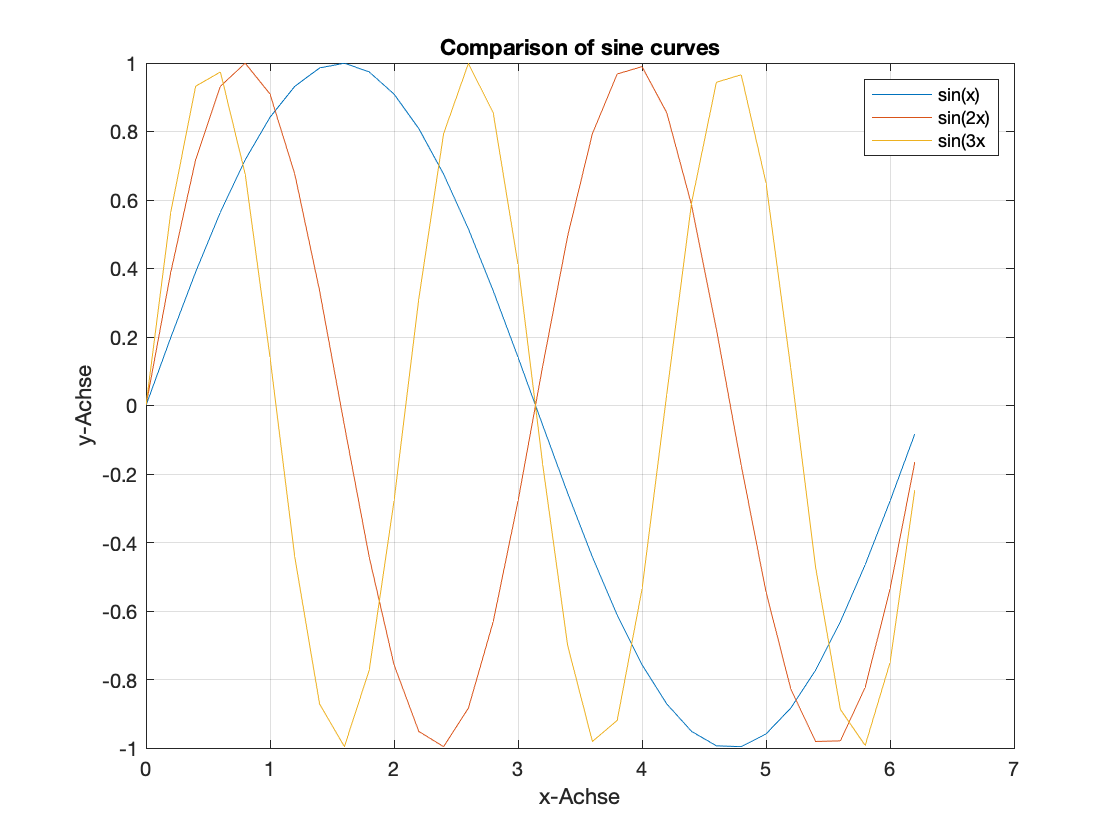
\includegraphics[scale=0.3]{../../PROJEKTE/ubungm2a/ubungm2a.png}
\end{center}
\item Stellen Sie diese Funktionen in einer neün Figure alle untereinander dar.
\lstinputlisting[language=Matlab, caption={übung M2b) Teil 2}]{../../PROJEKTE/ubungm2b/ubungm2b.m}
\begin{center}
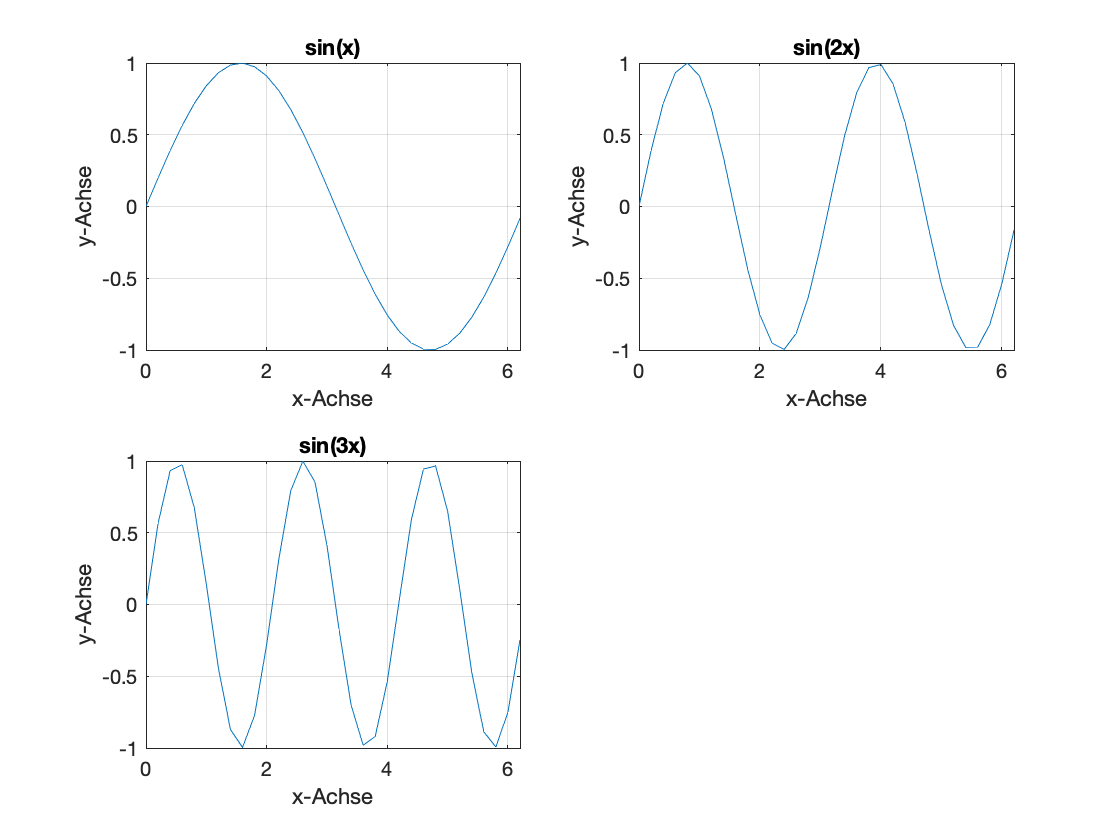
\includegraphics[scale=0.3]{../../PROJEKTE/ubungm2b/ubungm2b.png}
\end{center}
\item Stellen Sie $\texttt{e}^\texttt{x}$ und \texttt{ln(x)} in einer neün Figur dar.
\lstinputlisting[language=Matlab, caption={übung M2b) Teil 3}]{../../PROJEKTE/ubungm2c/ubungm2c.m}
\begin{center}
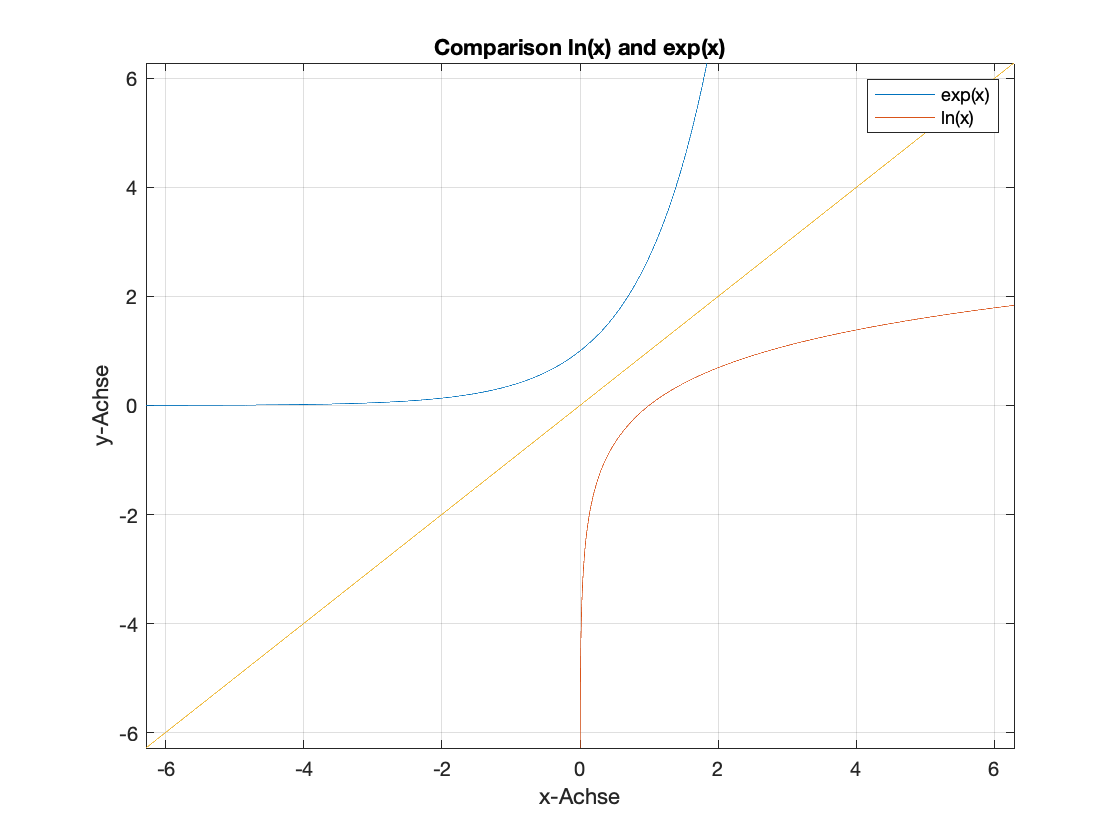
\includegraphics[scale=0.3]{../../PROJEKTE/ubungm2c/ubungm2c.png}
\end{center}
\end{enumerate}











\chapter{M3 Übung: Vektoren und Arrays, Funktionen}
\textbf{Drehbuch}
\begin{enumerate}
\item Fragen zum Buch.
\item Lernseqünz: Berechnung mittels Vektorisierung (geleitet).
\item übung 1: Wurfparabel (geleitet).
\item Kap. 6 (Funktionen und Fehlerhandling) vom Buch „Die nicht zu kurze Kurzeinführung in MATLAB“ selbstständig durcharbeiten.
\end{enumerate}
\textbf{Lernziele}
Die Studierenden...
\begin{enumerate}
\item festigen den Umgang mit Matlab.
\item erkennen, das viele Schleifen in Matlab nicht ausgeführt werden müssen.
\item verstehen die Mächtigkeit von Vektoroperationen.
\item und ebenso Darstellungsmöglichkeiten von ganzen Matrizen.
\item wissen, was ein m-File ist und können eine Funktion erstellen.
\end{enumerate}
\section{Wurfparabel}
Die Wurfparabel stellt den Verlauf eines Balles dar, der mit einer gewissen Anfangsgeschwindigkeit und einem gewissen Abschusswinkel geworfen wird.
Der Weg, den dieser Ball beschreibt, kann folgendermassen ausgedrückt werden:
\begin{equation}
sx\left(t\right)=\Big\vert\overrightarrow{v}\Big\vert\cdot \cos\left(\alpha\right)\cdot t
\end{equation}
\begin{equation}
sy\left(t\right)=\Big\vert\overrightarrow{v}\Big\vert\cdot\sin\left(\alpha\right)\cdot t-\dfrac{g}{2}\cdot t^2 
\end{equation}
$sx(t)$: $x$-Komponente der Wurfbahn [m].\\
$sy(t)$: $y$-Komponente der Wurfbahn [m].\\
$\Big\vert \overrightarrow{v}\Big\vert$ : Betrag der Wurfgeschwindigkeit [m/s].\\
$\alpha$: Abschusswinkel [grad, rad].\\
$t$: Zeit [s].\\
$g = 9.81$: Gravitationskonstante [m/s2
]\\\\
Programmieren Sie in MATLAB ein M-File, welches die Wurfparabel darstellt. Die Anzahl der
dargestellten Parabeln soll im M-File verändert werden können. Bei welchem Abschusswinkel
wird die Wurfweite maximal?  
\begin{center}
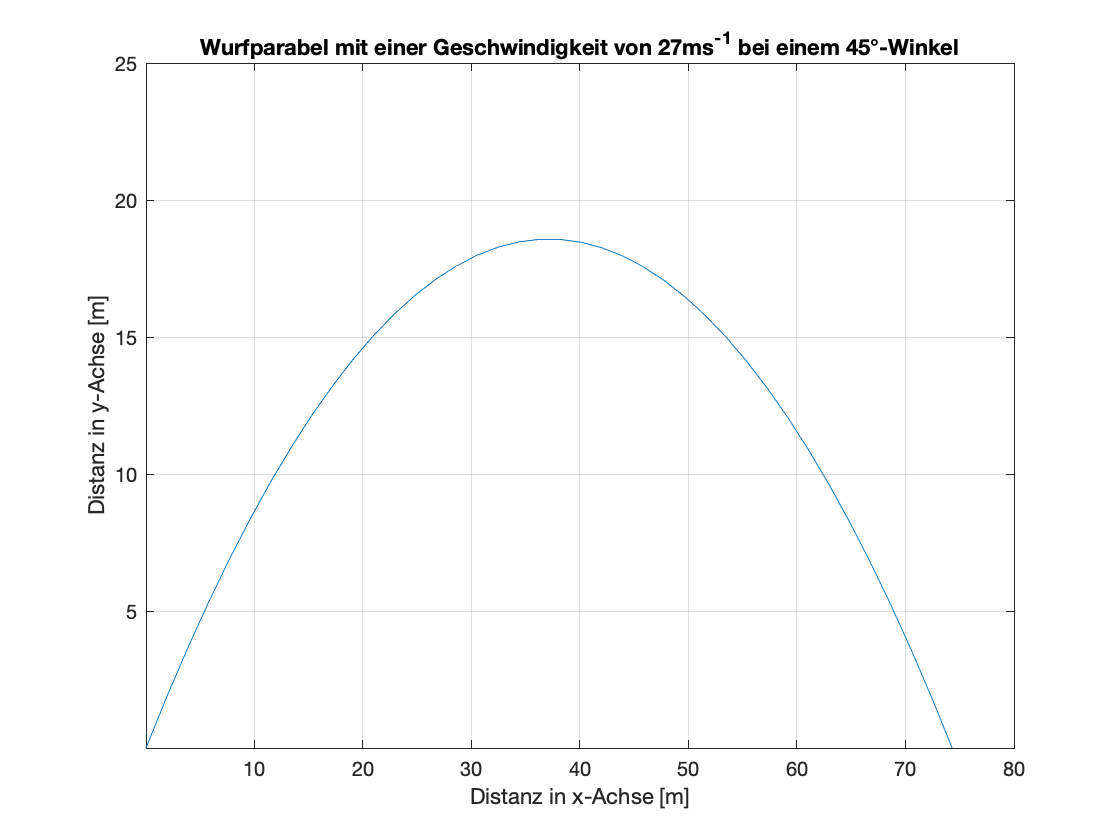
\includegraphics[scale=0.3]{../../PROJEKTE/ubungm3wurfparabel/ubungm3wurfparabel.png}
\end{center}
\lstinputlisting[language=Matlab, caption={Wurfparabel für 60 Grad}]{../../PROJEKTE/ubungm3wurfparabel/ubungm3wurfparabel.m}
\section{M3a) übung zu Funktionen}
öffnen Sie die Funktion {\color{magenta}\texttt{linspace}} mit dem Befehl {\color{magenta}\texttt{edit linspace}} und analysieren Sie diese Funktion von Mathworks. 
\lstinputlisting[language=Matlab, caption={übung M3a)}]{../../PROJEKTE/ubungm3a/ubungm3a.m}
Beantworten Sie folgende Fragen
\begin{enumerate}[$a)$]
\item Wie lang ist die Länge eines Standardvektors, wenn {\color{magenta}{keine Länge}} definiert wird?
\\
$\Longrightarrow$ Generierung eines Vektors mit 100 linear gleichabständigen Punkten.
\item Mit {\color{magenta}\texttt{help linspace}} erscheint die Hilfe dieser Funktion im Command Window 
\begin{enumerate}[$\bullet$]
\item Wo befindet sich dieser Text in der Datei?
\\
$\Longrightarrow$ Der angezeigte Text befindet sich im Command Window.
\item Ab welcher Zeile wird der Hilfetext nicht mehr ausgegeben? Wie wird dies abgegrenzt?
\\
$\Longrightarrow$ Eine Zeile vor der Zeile des Copyrights wird nichts mehr angezeigt. Durch {\color{magenta}\texttt{edit help}} kann man dies ändern.
\end{enumerate}
\end{enumerate}
\section{M3b) übung zu Kapitel 6}
Schreiben Sie eine Funktion welche die zwei Zahlen \texttt{a} und \texttt{b} addiert ({\color{magenta}\texttt{add}}), subtrahiert ({\color{magenta}\texttt{sub}}), multipliziert ({\color{magenta}\texttt{mult}}), dividiert ({\color{magenta}\texttt{div}}) und potenziert ({\color{magenta}\texttt{pow}}). Testen Sie diese Funktion gründlich. 
\lstinputlisting[language=Matlab, caption={übung M3a)}]{../../PROJEKTE/ubungm3b/ubungm3b.m}
\section{M3b) übung publish-pdf zu Kapitel 6}
Testen Sie Ihre Funktion nun selber, indem Sie die Testfunktion für die übung M3b) (oberhalb dieses Textblockes) herunterladen und mittels der Publish Funktion ausführen.
\\\\
Korrigieren Sie Ihre Funktion dual(a,b) so lange, bis keine Fehlermeldung mehr auftritt.
Einzig bei der Division durch Null kann es möglich sein, dass Fehler auftreten werden.
\\\\
Speichern auf Moodle folgende zwei Dateien ab:
\begin{enumerate}[$a)$]
\item Ein pdf von Ihrer Funktion dual(a,b)
\item Das Resultat der Publish Funktion (auch als pdf).
Der Code des Testfiles soll nicht eingebunden werden
\end{enumerate}



\end{document}
